\documentclass[nochap]{apuntes}

\newcommand{\theauthor}{}
\newcommand{\thetitle}{Criptografía y Seguridad Informática}
\newcommand{\rightheader}{Criptografía y Seguridad Informática}
\newcommand{\leftheader}{UAM - 2015/2016}

\title{Criptografía y Seguridad Informática}
\author{Cristina Kasner Tourné\\Jose Antonio García del Saz}
\date{15/16 C1}

% Paquetes adicionales

% --------------------
\usepackage{tikztools}
\usepackage{tikz-3dplot}
\usepackage{textcomp}
\usepackage{tikz-qtree}
\usepackage{changepage}
\usepackage{listings}
\usepackage{graphicx}
\usepackage{tikz}
\usepackage[all]{xy}
\usepackage{tikz-cd}
\graphicspath{ {Imagenes/} }
\begin{document}
\pagestyle{plain}
\maketitle

\tableofcontents
\newpage
% Contenido.
\chapter{Introducción criptografía y seguridad informática}
\section{ Definiciones básicas}

 \begin{defn}[Criptografía] Proviene de la palabra griega "oculto". Escribir de forma enigmática.
 \end{defn}
 
 
 \begin{defn}[Texto plano]
 	Texto original.El mensaje que se quiere cifrar está escrito en texto plano
 \end{defn}
 
 
 \begin{defn}[Texto cifrado]
	DIBUJO
 \end{defn}
 
 \begin{defn}[Estenografía]
 	Técnica para esconder mensajes dentro de otro mensaje.
 \end{defn}
 
 
 \section{Contexto histórico de la criptografía}
 
 \subsection{Principales motores de la criptografía}
 
 \begin{itemize}
 	\item Político\item Bélico \item Económico
 \end{itemize}
 
\section{Esquema general de cifrado y servicios proporcionados a la seguridad}

\section{Tipos de ataques}
\section{Modelos y estándares de seguridad informática, auditoría y certificación}

\chapter{Métodos clásicos de cifrado y criptoanálisis}
\section{Definición de criptosistema}
\begin{defn}[Criptosistema]
	Es una quíntupla $(P, C, K, E_k, D_k)$ que satisface
	
\begin{itemize}
	\item $P \rightarrow$ conjunto de textos planos
	\item $C \rightarrow$ conjunto dde textos encriptados
	\item $K \rightarrow$ claves
	\item $E_k(x) \rightarrow$ función de cifrado
	\item $D_k(x) \rightarrow$ función de descifrado
\end{itemize}

\end{defn}
\subsection{Cifrados alfabéticos}
\subsubsection{Cifrado de desplazamiento}

\begin{itemize}
	\item $P\in Z_m$
	\item $C\in Z_m$
	\item $K\in Z_m$
	\item $y=E_k(x)= x+k$ mod m, con $x\in Z_m$ y $K \in Z_m$
	\item $D_k(y) = x- k$ mod m
	
\end{itemize}

La complejidad de descifrado depende de $|K|$, en este caso
$$|K| = |Z_m| = m$$
Vemos que $E_k$ y $D_k$ son muy rápidas, por lo que se pueden ejecutar en tiempo real, pero a la vez es muy fácil de descifrar.

\subsubsection{Cifrado de sustitución}

\begin{itemize}
		\item $P\in Z_m$
		\item $C\in Z_m$
		\item $K \rightarrow$ permutación de símbolos
		\item $y=E_k(x)= \Pi(x)$ ($\Pi \rightarrow$ permutación)
		\item $D_k(y) = \Pi^{-1}(y)$
\end{itemize}

Es importante ver que en $Pi$ no puede haber índices repetidos.
\begin{example}
	
	
	\textbf{\\ \\ Bien:}
	
	$\begin{matrix}
		1 & 2 & 3 & 4\\
		2 & 1 & 3 & 4
	\end{matrix}$
	
	\textbf{\\ Mal:}
	
		$\begin{matrix}
		1 & 2 & 3 & 4\\
		1 & 1 & 3 & 4
		\end{matrix}$
	
	
\end{example}

Este cifrado es más complejo ya que $|K| = m!$

\subsubsection{Cifrado afín}

\begin{itemize}
	\item $P\in Z_m$
	\item $C\in Z_m$
	\item $K \in (a,b)$
	\item $y=E_k(x)= ax + b$ mod $m , a\in Z^*_m$ y $b\in Z_m$
	\item $D_k(y) = (y-b)* a^{-1}$ mod $m$
\end{itemize}

Decimos que $ a\in Z^*_m$ ya que si $ a\in Z_m$, entonces $a^{-1}$ no tiene porqué existir. Por esto definimos
$$Z^*_m = \{a\in Z_m | mcd(m,a) = 1\}$$

Esto nos asegura que $\forall a \in Z^*_m $ existe $a^{-1}$

Para saber que $a$ queremos utilizar, tenemos que ver:
\begin{enumerate}
	\item mod(a,m) = 1. Para comprobar esto utilizamos el algoritmo de Euclides.
	
	\item ¿Cómo hallamos $a^{-1}$? . Para esto utilizaremos el algoritmo de Euclides extendido.
\end{enumerate}

\begin{enumerate}
	\item \textbf{mcd(a,m) = mcd(m, a mod m)}\\
	
	
	\underline{EUCLIDES}
	
	Llamamos $r_0 = a$ y $r_1 = m$
	
	$r_0 = q_1 r_1 + r_2$, de forma que $mcd(r_0,r_1) = r_2$
	
	$r_1 = q_2 r_2 + r_3$
	
	$\dots$
	
	$r_{n-2} = q_{n-1}r_{n-1} + r_n$
	
	$r_{n-1} = q_{n}r_{n}$
	
	Y asi nos queda que
	$$r_n = mcd (a,m)$$
	
	\item \textbf{¿ $a^{-1}$?}\\
	
	\underline{EUCLIDES EXTENDIDO}
	
	La idea es escribir el algoritmo de Euclides pero escribiendo todos los restos en función de $a$ y $m$.
	
	Llamamos $r_0 = a$ y $r_1 = m$
	\begin{itemize}
		\item $r_0 = q_1 r_1 + r_2 \implies r_2 = r_0 - q_1 r_1 \implies r_2 = a-q_1m$
		
		\item $r_1 = q_2 r_2 + r_3 \implies r_3 = m - q_2 r_2$ , y como $r_2$ está e función de $a$ y de $m$ , entonces $r_3 = m(1+q_1q_2) - q_2a$
		
		\item $r_4 = r_2 - q_3 r_3$
		
		$\dots$
		
		\item $r_{n} = m\cdot U_n + a\cdot V_n \implies a \cdot V_n = 1$ mod $m \implies a^{-1} = V_n$
		
	\end{itemize}
	
	Ejercicio: ¿Cómo calculamos esa $V_n$?
	
	 $r_0 = r_0$\\ $r_1 = r_1$\\$r_2 = r_0 -q_1r_1$\\$r_3 = -q_2r_0 + (1+q_1q_2)r_1$\\ $r_4 = (1+ q_3q_2)r_0 -(q_1 +q_3(1+q_2q_1))r_1$\\ ... \\ Llamamos al término que acompaña al $r_0$ : $U_i$ y al término que acompaña al $r_1$ : $V_i$\\ 
	 
	 Para calcular $U_i$ cogemos $U_0=1$ , $U_1 = 0$ y calculamos:
	 $$U_i = U_{i-2} - q_{i-1}U_{i-1} \iff i\geq 2$$
	
	 Para calcular $V_i$ cogemos $V_0=0$ , $V_1 = 1$ y calculamos:
	 $$V_i = V_{i-2} - q_{i-1}U_{i-1} \iff i\geq 2$$
	 
	 \begin{example}
	 Euclides (a,b)	 
	 	
	 	$r_0 \leftarrow a$\\$r_1\leftarrow b$\\$m\leftarrow 1$
	 	
	 	while $r_m \neq 0$
	 	
	 	 do 
	 	$\begin{cases}
	 		q_m \leftarrow \lfloor\frac{r_{m-1}}{r_m}\rfloor\\ r_{m+1} \leftarrow r_{m-1} - q_mr_m\\m\leftarrow m +1
	 		
	 	\end{cases}$
	 	
	 	$m\leftarrow m-1$
	 	
	 	return ($q_1,...,q_m; r_m$)
	 \end{example}
	 
\end{enumerate}
 \begin{theorem}[Teorema Fundamental de la Aritmética]
 	Todo número se puede descomponer en un producto de números primos.
 	$$m = \Pi^{n}_{i-1} \cdot p^{e_i}_{i}$$
 	
 \end{theorem} 
 
 \begin{theorem}[Función de Euler]
 	La función de Euler nos indica el número de coprimos a uno dado.
 	$$\phi(m) = |Z^{*}_m| = \Pi{n}_{i=1} (p^{e_i}_i - p^{e_i-1}_i)$$
 	
 \end{theorem}
 

 
 \begin{example}
 	Vamos a buscar cuantas claves tenemos en español (27 letras)
 	$$K = |Z_{27}| x |Z^{*}_{27}| = 27\cdot 18 = 486$$
 \end{example}


Vamos a ver una forma de calcular el inverso multiplicativo con Euler generalizado, esta forma no vale para números grandes.

\begin{theorem}[Euler generalizado]
	$$\text{a} \in Z^{*}_m \implies a^{\phi(m)} \equiv 1 \text{ mod } m$$
\end{theorem}

\textbf{Truco para inverso}:

$$a^{\phi(m)} = a^{\phi(m) - 1} \cdot a \equiv 1 \text{ mod } m$$
$$...$$
$$a^{\phi(m) -1} = a^{-1} \text{ mod } m$$

\textbf{¿Porqué no se utiliza esta forma de calcular en inverso?} Porque necesitamos $\phi(m)$ , que se calcula con la descomposición en números primos, y esto no es trivial para números grandes.

Hasta ahora hemos estado viendo cifrados alfabéticos, es decir, que vamos cifrando cada letra del mensaje plano con una clave, de forma que nos queda el mensaje cifrado.


A partir de ahora vamos a ver cifrados en bloque

\subsection{Cifrados en bloque}

\subsubsection{Cifrado de Vigenere}

\begin{itemize}
	\item $P= Z_m \times Z_m \times ..... \times Z_m = (Z_m)^{n}$
	\item $C = (Z_m)^{n}$
	\item $K = (Z_m)^{n} = P = C$
	\item $E_{\overrightarrow{k}} = E_{k_1,...,k_n}(\overrightarrow{x}) = (x_1+ k_1,...,x_n+ k_n) \text{ mod } m \equiv Y$
	\item $D_{k_1,...,k_n} ( \overrightarrow{Y}) = (y_1- k_1,...,y_n- k_n) \text{ mod } m $
\end{itemize}

\subsubsection{Cifrado de Hill}

\begin{itemize}
	\item $P= (Z_m)^{n}$
	\item $C = (Z_m)^{n}$
	\item $K$ es una matriz $n \times n$
	\item $\overrightarrow{y} = E_{k}(\overrightarrow{x}) = (x_1,....,x_n) \cdot K \text{ mod } m$
	\item $D_{k}(\overrightarrow{y})= (y_1,....,y_n) \cdot K^{-1}_{n \times n}$
\end{itemize}
\paragraph{Condiciones para este criptosistema}
\begin{enumerate}
	\item det($K$)$\neq 0$ $\implies$ esto es para que exista $K^{-1}$
	\item mcd (det($K$) , $m$)$= 1$
\end{enumerate}

\subsubsection{Cifrado de permutación}
\begin{itemize}
	\item $P= (Z_m)^{n}$
	\item $C = P$
	\item $K$ es un vector de permutación $\overrightarrow{\Pi}$ de n permutaciones
	\item $E_{k}(\overrightarrow{x}) = (x_{\Pi(1)},....,x_{\Pi(n)})= Y$
	\item $D_{k}(\overrightarrow{y})= (y_{\Pi(1)},....,y_{\Pi(n)}$
\end{itemize}

\begin{example}
	
	$n=6$
	
	$$\begin{matrix}
	x = & 1 & 2 & 3 & 4 & 5 & 6\\
	\Pi(x) = & 3 & 5 & 1 & 6 & 4 & 2\\
	\end{matrix}$$
	
	$$\begin{matrix}
	y = & 1 & 2 & 3 & 4 & 5 & 6\\
	\Pi(y)^{-1} = & 3 & 6 & 1 & 5 & 2 & 4\\
	\end{matrix}$$
\end{example}

Es muy sencillo transformar un \textit{Cifrado de Permutación} en un \textit{Cifrado de Hill}. Vamos a ver como:

\begin{example}
	
	Estamos en $Z^3_n$ , la permutación es $\Pi = (3,2,1)$.
	
	$\begin{matrix}
		x\rightarrow & 1 & 2 & 3\\
		\Pi(x)\rightarrow & 3 & 2 & 1\\
	\end{matrix} \iff \begin{matrix}
	(x_1 & x_2 & x_3)
	\end{matrix} \left(\begin{matrix}
		0 & 0 & 1\\ 0 & 1 & 0\\ 1 & 0 & 0
	\end{matrix}\right) = \begin{matrix}
	(x_3 & x_2 & x_1)
	\end{matrix}$
\end{example}

\subsection{Cifrados de flujo}

Hay dos tipos de cifrados de flujo:
\begin{itemize}
	\item \textbf{Síncronos} $\rightarrow$ K independiente de M
	\item \textbf{Asíncronos} $\rightarrow$ si K depende de las claves anteriores
\end{itemize}

En este tipo de cifrado la transformación va a ser del tipo:

$\begin{matrix}
 X \sim & X_1 & X_2 & ....\\
 Z \sim & Z_1 & Z_2 & ....\\
\end{matrix} \implies \begin{matrix}
y \sim & e_{Z_1}(x_1) & e_{Z_2}(x_2) & ....\\
\end{matrix}$

\begin{example}[Cifrado síncrono de flujo periódico de periodo d]
	\begin{itemize}
		\item $P= C = Z_n$
		\item $e_Z(x) = x + Z$ mod $m$
		\item $d_Z(x) = x - Z$ mod $m$
		\item $Z \rightarrow$ es el flujo de claves $\implies Z = Z_1Z_2...$
		
		$Z_i \begin{cases}
			K_i \text{ si } 1 \leq i \leq 1\\
			Z_{i-n} \text{ si } i \geq n+1
		\end{cases}$ 
		
		Al ser cifrado de flujo periódico de periodo d $\implies Z_{i+d} = Z_i$ 
	\end{itemize}
	\begin{remark}
		El los \textbf{Alfabetos binarios},  $e_Z(x) = x + Z$ mod $2$ , que es lo mismo que hacer un XOR
	\end{remark}
\end{example}




\subsubsection{Generador de claves}

 Para obtener seguridad en los dispositivos hardware , se emplean registros de desplazamiento retoralimentados como generadores de números pseudoaleatorios para las claves de cifrados de flujo.
 
 Estos registros pueden ser:
 
\begin{itemize}
	\item LFSR $\rightarrow$ registros de desplazamiento con retroalimentación lineal
	\item NLFSR $\rightarrow$ registros de desplazamiento con retroalimentación no lineal
\end{itemize}

Con esto generamos una \textbf{key stream}.

\textbf{¿Cómo funciona?}
\begin{enumerate}
	\item Primero generamos una clave : $Z_i = K_i$  $1< i \leq n$ ; $c = (c_0, c_1....c_{n-1}) \implies K = (K_1, K_2,..., K_n,c_0....c_{n-1})$
	\item Recurrencia (de orden n). Un ejemplo es
	$$Z_{i+n} = \sum_{j=0}^{n-1} c_j \times Z_{i+j} \text{ mod } 2$$
\end{enumerate}

\begin{example}[RC4]
	\begin{center}
		\Tree[.ClaveSecreta [.RC4 [.KeyStream [.Tp$\to\oplus\to$Tc ] ] ] ]
	\end{center}
\end{example}

\begin{problem}
	Hallar el orden de recurrencia de la siguiente clave:
	$$(1000,1100)$$
	
	\solution Se deja como ejercicio para el lector. El orden deberá salir 15.
	
\end{problem}

\subsection{Producto de Criptosistemas}
Se define de la siguiente forma:


	$S_1 = [ P, C, K_1 E_{K_1} D_{K_1}]$
	
	$S_2 = [ P, C, K_2 E_{K_2} D_{K_2}]$
	
	$$S_1 \times S_2 = [ P, C, K_1 E_{K_1} D_{K_1}] \times [ P, C, K_2 E_{K_2} D_{K_2}] = [ P, C, K_1 \times K_2, E_{K_1 K_2} D_{K_1 K_2}]$$
	
	\begin{problem}
		Combina los siguientes criptosistemas:
		$$\begin{cases}
		 y = x + K_1 \text{ mod } m\\
		 y = x + K_2 \text{ mod } m\\
		\end{cases}$$
		\solution
		$E_{K_2}(E_{K_1}(x)) = E_{K_2}(x + K_1) = x + K_1 + K_2$
	\end{problem}
	
	\begin{problem}
		Combina los siguientes criptosistemas y halla la robusted del criptosistema resultante
		$$\begin{cases}
		y = x + b\\
		y= ax\\
		\end{cases}$$
		
		\solution
		\begin{itemize}
			\item $E_{K_2}(E_{K_1}(x)) = E_{K_2}(x + b) = a \cdot(x + b) = ax + ab$
			
			Como $ab \in Z_m$ llamamos $ab = \beta \in Z_m$ de forma que el producto de los criptosistemas nos queda:
			$$ax + \beta \text{ mod } m$$
			\item Para calcular la robusted vemos que 
			\begin{itemize}
				\item $|b| = m$
				\item $|a| = |Z^{*}_m| = \phi(m) \text{ mod } m$
			\end{itemize}
			Ahora ya podemos calcular la robusted del producto
			$$|a| \cdot |\beta| = |Z^{*}_m| \cdot |Z_m| = \phi(m) \cdot m$$
		\end{itemize}
			
	\end{problem}
	
\begin{remark}
Combinar cifrados de sustitución con permutación ha dado lugar a cifrados como : \textbf{CRIPITO, DES, AES...} 
\end{remark}

\section{Tipos de ataques}

\subsection{Criptoanálisis}
En el criptoanálisis el algoritmo es conocido.

Del criptoanálisis deriban las \textbf{Reglas de Kerchhoffs}
\begin{enumerate}
	\item Algoritmo de cifrado público
	\item La fortaleza del criptograma reside en K(clave)
\end{enumerate}

Vamos a ver los supuestos ataques con los que podeos encontrarnos

\begin{itemize}
	\item[A)] Solo texto cifrado $\rightarrow$ es el caso más difícil.
	\item[B)] Texto claro conocido $\rightarrow$ texto cifrado + pareja plano-cifrado 
	\item[C)] Texto claro elegido $\rightarrow$ texto cifrado + pareja plano elegida-cifrado
	\item[D)] Texto cifrado elegido $\rightarrow$ texto cifrado + pareja plano-cifrado elegido 
	\item[E)] Texto elegido 
\end{itemize}

\subsubsection{Cifrado de desplazamiento}

Este cifrado se rompe de forma \textbf{inmediata} en los supuestos \textbf{B, C, D} y \textbf{E}.

En el caso \textbf{A} no es inmediato pero también es sencillo. Se hace utilizando las estadísticas del idioma.

\begin{example}[Supuesto A-] 
	
	Sabemos que la letra que más se usa en el español es la E ($16'.. \%$) , si en nuestro texto cifrado la letra más repetida es la D, es lógico pensar que $e_K(E) = D$.
	
	A partir de aquí es fácil hallar la clave.
	
	Si vemos que el resultado es un texto sin sentido, cambiaremos nuestra hipótesis(en función de las estadísticas) y seguiremos probando.
\end{example}


\subsubsection{Cifrado Afín}

Este cifrado se rompe de forma \textbf{muy sencilla} en los supuestos \textbf{B, C, D} y \textbf{E} si tengo dos parejas de texto plano-cifrado (x-y)
$$\begin{cases}
x_1 - y_1\\
x_2 - y_2
\end{cases} \rightarrow \begin{cases}
y_1 = x_1 + b \text{ mod }m\\
y_2 = x_2 + b \text{ mod }m\\
\end{cases}$$
Y resuelvo el sistema.

En el caso \textbf{A} no es tan sencillo pero con estadística también se puede romper. Si la primera hipótesis falla, probaremos con la siguiente letra más probable hasta dar con un texto que tenga sentido.

\subsubsection{Cifrado de Sustitución}

Este es más complicado, necesitaremos estadísticas más completas (COMPLETAR DEL LIBRO)

\subsubsection{Cifrado de Vigenere}

$$\overrightarrow{y} = \overrightarrow{x} + \overrightarrow{K} \text{ mod } m$$

Para analizar esto una simple estadística no vale, porque dependiendo de cual sea  la longitud de la clave, \textbf{mismos textos se cifran de forma diferente}.

Por lo tanto el criptoanálisis se hace en dos pasos:
\begin{enumerate}
	\item\textbf{ Hallar el tamaño de la clave $\rightarrow$ ¿n?}
	
	Para esto podemos utilizar dos métodos $\begin{cases}
	KASISKI \rightarrow 1863\\
	\textit{Índice de coincidencia}\\
	\end{cases}$
	\begin{itemize}
		\item \textbf{KASISKI} $\rightarrow$ Se basa en la suposición de que puede haber repeticiones en el texto cifrado que vengan de la misma parte del texto plano.
		
		\begin{enumerate}
			\item localizamos las repeticiones y las llamamos $Y_1$
			\item llamamos a la posición de inicio de cada repetición $i_1, i_2,i_3...$
			\item llamamos la distancia entre las repeticiones $\delta_1 , \delta_2....$
			\item vemos que :
			
			$\begin{cases}
			i_2 = i_1 + K_1\cdot n\\
			i_3 = i_2 + K_2\cdot n\\
			....\\
			\end{cases}$ 
			
			COMPLETAR!!!!
		\end{enumerate}
		\item \textbf{Índice de coincidencia} $\rightarrow$ Dado una cadena de datos $\overrightarrow{X} = X_1 X_2 .... X_l$, el índice de coincidencia de dicha cadena $I_c(\overrightarrow{X})$ es la probabilidad de que dos elementos de esa cadena coincidan.
		
		Supongamos que tenemos una serie de caracteres en $\overrightarrow{X}$ con frecuencias de ocurrencia $f_0,f_1, f_2 ....$.
		
		Nos preguntamos: ¿De cuantas formas podemos combinar un caracter $X_i$ en dicha cadena?
		$$\comb{f_i}{n}$$
		¿De cuantas formas podemos coger n $X_i$ iguales?
		$$\sum_{i} \comb{f_i}{n}$$
		
		\begin{remark}
			Supongamos que tenemos n objetos y queremos elegir los objetos de $r$ en $r$ sin atender a la ordenación de los mismos.
			
			El número de combinaciones que existen de n objetos tomados de $r$ en $r$ es $\comb{r}{n}$
		\end{remark}
		

		
		Por lo tanto el caso de mayor $I_c(X)$ es el caso en que la cadena tenga todos los caracteres iguales.
		
		Una vez visto todo esto podemos definir el $I_c(X)$ como:
		$$I_c(\overrightarrow{X}) = \frac{\sum_{i}\comb{f_i}{2}}{\comb{l}{2}} = ... = \frac{\sum_{i} f_i \cdot (f_i -1)}{l\cdot(l-1)} = \sum_{i} \frac{f_i}{l} \cdot \frac{f_i-1}{l-1} $$
		
		Si nos fijamos:
		
		$\frac{f_i}{l} = P_i$ es la probabilidad de cada letra y $\frac{f_i-1}{l-1} \sim P_i$, por lo tanto
		$$I_c(\overrightarrow{X}) \sim \sum_{i} P^2_i$$
		
		Este índice lo hemos calculado para los 1-gramas.
		
		\begin{defn}[n-grama]
 composición de n símbolos de un lenguaje
		\end{defn}
		
		\begin{example}
			Vamos a ver el índice de coincidencia de un lenguaje aleatorio y el del inglés:
			$$I_c(\overrightarrow{X})_{aleatorio} = 0.038$$
			$$I_c(\overrightarrow{X})_{inglés} = 0.065$$
		\end{example}
		
		
	\textbf{Y con esto, ¿cómo calculamos el número de claves?}
	
	\begin{example}
		
		Tamaño de $\overrightarrow{K} = n$ ,	$\overrightarrow{K} = \{K_1, K_2, ....\}$
		Sabemos que estamos en el cifrado de Vigenere.
		
		\textbf{Pregunta: ¿n?}
		
		Vamos a hallarla con el $I_c(\overrightarrow{x})$
		
		$$M_c = y_1...y_n' , y_{n'+1}.....y_{2n'} , y_{2n'+1}....y_{3n'},....y_l$$
		
		$$\begin{cases}
			\overrightarrow{X_1}= y_1, y_{n'+1}, y_{n'+2}...\\
			\overrightarrow{X_2}= y_2, y_{n'+2}, y_{2n'+2}...\\
			.....\\
			\overrightarrow{X_n}= y_{n'}, y_{2n'}, y_{3n'}...\\
		\end{cases}$$
		
		¿Cómo sabemos si $n' = n$? Podemos ir probando con diferentes $n'$, el correcto será el que de un $I_c$ similar al del lenguaje en el que esté el mensaje en claro.
	\end{example}
	
	\end{itemize}
	\item \textbf{Descubrir las $K_i$}
	
	Para esto también podemos utilizar el $I_c$.
	
	\textit{\textbf{La idea es:} Si mi clave es de longitud 3, cojo el mensaje cifrado y cojo los caracteres 1,4,7,10...(esto es $X_1$) y sabemos que todos esos caracteres han sido cifrados con la misma letra. Ahora vamos probando distintas letras (claves), sobre dichos caracteres y calculamos su $I_c$, de nuevo cuando el $I_c$ coincida con el del idioma en el que está escrito el mensaje, tendremos la clave correcta. Hacemos esto con cada $X_i$}
	
	Lo primero que hacemos es calcular todas las frecuencias de esa cadena, $f_j : 0 \leq j < m$
	
	Vemos que la longitud de cada $\overrightarrow{X}_i$ es $\frac{l}{n}$ y el número de símbolos del lenguaje es $m$
	
	$$I_c(\overrightarrow{X}) = \sum_{j=0}^{m-1} p_j \cdot \frac{f_{j-K_i}}{\frac{l}{n}} = M(K_i)$$
	
	$$M_g = \sum_{j=0}^{m} p_j \frac{f_{j+g}}{l/n} = M(K_i)$$ 
	\begin{example}
		
		Contrastar que $\sum_{i}^{m-1} p_i p_{i-l} = \sum_{i}^{m-1} p_i p_{i+l}$
		
	\end{example}
	
	\begin{problem}[5]
		Probar que $y = a\cdot b$ mod $m$ constituye un criptosistema siempre y cuando $mcd(a,m) = 1$
		
		\solution
		Vamos a suponer 2 casos:
		
		\underline{CASO 1} : $mcd(a,m) = 1$
		$$\begin{cases}
		y_1 = ax_1 + b\\y_2= ax_2 +b
		\end{cases} \implies a(x_1 - x_2) = 0 \text{ mod } m $$
		
		Entonces
		
		$$a(x_1 - x_2) = q \cdot m \implies q = \frac{a(x_1 -x_2)}{m}$$
		
		tal que m \textbf{no divide} a $a$ $\implies m>a$
		
		También vemos que m \textbf{no divide} a $x_1 - x_2$ ya que ambos pertenecen a $Z_m$ por lo tanto ambos serán más pequeños que $m$.
		
		
		
		\underline{CASO 2} : $mcd(a,m) = d > 1$ de forma que $d$ divide a $a$ y $m$.
		
		$a(x_1 - x_2) = 0 \text{ mod } m$
		
		Llamamos $a_d = \frac{a}{d}$ y $m_d = \frac{m}{d}$
		
			$$a(x_1 - x_2) = q \cdot m \implies a_d(x_1 - x_2) = q \cdot m_d$$
			
			$$q = \frac{a_d(x_1 -x_2)}{m_d}$$
			
			Vemos que $m_d$ no divide a $a_d$ porque $m_d > a_d$
			
			¿Puede dividir $m_d$ a $(x_1-x_2)$ ?  Si, porque $m_d <m$
		
	\end{problem}
	
\end{enumerate}
 \subsubsection{Cifrado de Hill}
 
 \begin{problem} Ejercicio 9 del libro
 	
 	Vamos a calcular el número de claves en el criptosistema de Hill.
 	
 	Supongamos que la matriz
 	$$M_K = ( \begin{matrix}
 	K_{11} & K_{12}\\
 	K_{21} & K_{22}
 	\end{matrix} ) $$
 	
 	Determinante de $M_K \neq 0$ , mcd(det($M_K$),$P$)$= 1$ , siendo $P$ primo.
 	\solution
 	
 	Vemos que cuando $P$ es primo y det$\neq 0$, siempre se cumple que son coprimos.
 	
 	
 	
 \end{problem}
 
 % % Parte de Jose
 
 \chapter{Cifrado perfecto y distancia de unicidad}
 
 \textbf{1949}$\rightarrow$ Sientan las bases teóricas del cifrado automático (Claude Shannon).
 
 \section{Seguridad perfecta}
 
 En este capítulo veremos dos temas, siempre basándonos en que nos encontramos en el \textbf{caso A} (solo tenemos el texto cifrado).
 
 \begin{itemize}
 	\item \textbf{SEGURIDAD PERFECTA}
 	\begin{itemize}
 		\item \textbf{Seguridad Computacional}
 		\begin{itemize}
 			\item Análisis que se hace a los algoritmos criptográficos para ver cómo romperlos.
 			\item  Intenta aproximar cuantas operaciones necesitas hacer para poder romper el sistema(averiguar la clave).
 			\item Un buen criptosistema es quel cuyo tiempo de uso es mucho menos que el tiempo que necesitamos para romperlo.
 			
 		\end{itemize} 

 		\item \textbf{Seguridad incondicional}
 		\begin{itemize}
 			\item Modelo en el que tenemos una máquina con recursos ilimitados, esta no es capaz de romper el criptosistema.
 		\end{itemize}
 	\end{itemize}
 	
 \end{itemize}


\begin{remark}
	Antes de seguir con segurdad perfecta vamos a repasar algunos conceptos de probabilidad que nos serán utiles en el estudio de este tema.
	
	Tenemos $x \in X = \{ x_1,....x_n\} , y \in Y = \{ y_1,...y_n\}$
	
	Llamamos $P(x = x_1) = P_p(x)$ y $P(y = y_1) = P_c(y)$
	
	Probabilidad conjunta:
	
	$$P(x,y) = P(x|y)\cdot P(y)$$
	
	y calculamos $P(x|y)$ de la siguiente forma:
	$$P(x|y) = \frac{P(x,y)}{P(y)} = \frac{P(y|x) \cdot P(x)}{P(y)} = \frac{P(y|x) \cdot P(x)}{\sum_{x} P (y|x)P(x)}$$
	
	
	Ahora vamos a aplica esto a los criptosistemas:
	
	$$P_p(x) ; x \in P \rightarrow\text{  P = texto plano}$$
	$$P_k(k) ; k \in K \rightarrow\text{  K es el conjunto de claves}$$
	
	Si tenemos independencia entre x y k $ \implies P(x,k) = P_p(x)P_k(k)$
	
	¿Y como calculamos $P_c(y)$?
	
	$$P_c(y) \underbrace{=}_{\text{bayes}} \sum_{k}P(x,k,y) = \sum_{xk} P(y|xk) \cdot P(xk) \underbrace{=}_{\text{IE}} \sum_{xk} P(y|xk)P_p(x) P_k(k)$$
	
	$$P(y|xk) = \begin{cases}
		\text{Si } e_k(x) = y \implies P(y|xk) = 1\\
		\text{Si } e_k(x) \neq y \implies P(y|xk) = 0\\
	\end{cases} \implies \textbf{Esto es la condición de criptosistema}$$
	
	Por lo tanto:
	$$\sum_{\forall x,y,k| y = e_k(x)} P_p(x) \cdot P_k(k) = P_c(y)$$
	
	Vamos a ver como se calcula la \textbf{probabilidad a priori}
	$$P_c(y|x) = \frac{P(y,x)}{P_p(x)} = \frac{\sum_{k}P(y,x,k)}{P_p(x)} = \frac{\sum_{k}P(y|kx)\cdot P(xy)}{P_p(x)} =$$
	 $$ =\frac{\sum_{k}P(y|kx)\cdot P_p(x)P_k(k)}{P_p(x)} = \sum_{k}P(y|kx)\cdot P_k(k)$$
	$$ \sum_{\forall k | e_k(x)=y} P_k(k) = P_c(y|x)$$
	
	Y ahora la \textbf{probabilidad a posteriori}
	$$P_c(x|y) = \frac{P_p(x) P_c(y|x)}{P_c(y)} = \frac{P_p(x) \sum_{\forall k| e_k(x) = y}P_k(k)}{\sum_{\forall x,k| e_k(x) =y} P_p(x) P_k(k)}$$
	
\end{remark}

\begin{defn}[Seguridad Perfecta]
	Decimos que un criptosistema tiene seguridad perfecta si cumple:
	$$P_p(x|y) = P_p(x)$$
	Esto quiere decir que el conocimiento de texto cifrado no nos da ninguna información sobre el texto plano.
\end{defn}

 Si tuvieramos el texto plano seria muy facil romperlo, pero tenemos que recordar que seguimos estando el el supuesto A (solo texto cifrado).

\begin{example}
	Supongamos que tenemos un texto plano $P=\{a,b\}$ tal que $P(a = 1/4)$ , $P(b) = 3/4$.
	
	Tenemos $K=\{k_1,k_2,k_3\}$ tal que $P(k_1) = 1/2$ , $P(k_2) = P(k_3) = 1/4$ y $c = \{1,2,3,4\}$

	
\begin{center}
		
	\begin{tabular}{l | c  r}
		  & a & b\\
		\hline
		$k_1$ & 1 & 2 \\
		$k_2$ & 2 & 3 \\
		$k_3$ & 3 & 4 \\
	\end{tabular}
\end{center}
	
		¿Cumple la seguridad perfecta?
		
		Vamos a calcular la probabilidad de que me salga cada uno de los elementos del texto cifrado:
	
	$$P_c(1) = P_p(a) P_k(k_1) = 1/8$$
	$$P_c(2) = P_p(a) P_k(k_2) + P_p(b) P_k(k_1) = 7/16$$
	$$P_c(3)= 1/4$$
	$$P_c(4) = 3/16$$
	Ahora vamos a mirar la probabilidad a priori de ese texto cifrado:
	
	$$P_c(1|a) = P_k(k_1) = 1/2$$
	$$P_c(2|a) = P_k(k_2) = 1/4$$
	$$P_c(3|a) = P_k(k_3) = 1/4$$
	$$P_c(4|a) = P_k(k_4) = 0$$
	
	$$P_c(1|b) = 0$$
	$$....$$
	
	y asi todo el rato
	
	Vamos a por la posteriori:
	$$P_p(a|1) = \frac{P_c(1|a) \cdot P_p(a)}{P_c(1)} = 1$$
	$$P_p(a|2) = \frac{1/16}{7/16}$$
	
	y asi todo el rato...
	
	Podeos ver que no es un criptosistema con seguridad perfecta.
\end{example}


\begin{example}
 	

Supongamos m claves del cifrado de desplazamiento que se que se ... con $P_k(k) = 1/m$ para cualquier $P_c(k)$

$$|P| , |C| , |K| = m$$

	\begin{center}
		
	\begin{tabular}{l | c | r}
		k|x & 0 & 1\\
		\hline
		0 & 0 & 1 \\
		\hline
		1 & 1 & 0\\
	
	\end{tabular}
\end{center}
	
	$$P_c(y) = \sum_{x,k | e_k(x) = y} P_p(x) P_k(x) = \frac{1}{m} \sum_{x|e_k(x) = y} P_p(x) = \frac{1}{m} \sum_{x=0}^{m-1} P_p(x) = \frac{1}{m} = P_c(y)$$


	$$P_c(y|x) = \sum_{k|e_k(x) = y; y= x+k} P_k(k) = \frac{1}{m}$$
	
	Y ya lo tenemos porque ahora podemos hacer la condicionada.
	
	$$P(x|y) = \frac{P(y|x) P (x)}{P(y)} = \frac{P(x) 1/m}{1/m} = P(x)$$
 \end{example}
 
 El criptosistema utilizado en el ultimo ejemplo es el \textbf{cifrado de vernan u OTP(one-time pad)}
 
 
 
 \underline{\textbf{Cifrado de OTP}}
 \begin{center}

 $M_p = x_1,....,x_n$\\
 $K= k_1,...,k_n \rightarrow P(k_1) = \frac{1}{k}$\\
 $M_c = y_1,...,y_n ; y_i = x_i + k_i$\\
 $|P| = |C| = |K| = m$
  	
  \end{center}
 
 Cuando se utilizaba este cifrado mandaban el mensaje por un canal inseguro y la clave por un canal seguro
 
 $$E \rightarrow P \rightarrow x+k = y \rightarrow \text{Canal Inseguro} \rightarrow Receptor$$
 $$\text{Generador de Claves} \rightarrow k \rightarrow \text{Canal Seguro} \rightarrow Receptor \rightarrow y-k \rightarrow P$$
 
 \begin{theorem}[Teorema cifrado perfecto]
 	Dado $[P,C,K,E_K,D_K]$ donde $|P| = |C| = |K|$ este proporciona seguridad perfecta si y solo si:
 	\begin{enumerate}
 		\item $P_k (k) = \frac{1}{|k|} ,  k\in K$
 		\item $\forall x \in P , \forall y \in C$ hay una sola clave tal que $e_k(x) = y$
 	\end{enumerate}
 \end{theorem}
 
 PROBLEMA PARA CASA: demostrar el teorema.
 
 Hay criptosistemas que no cumplen el teorema y son perfectos, como el afin, en el que las cardinalidades no son iguales.
 
 \section{Claves espúreas y distancia de unicidad}
 
 Ahora vamos a cifrar con una sola clave muchos mensajes.
 
  ¿Porqué esto es importante? Porque si los bloques son muy pequeños por probabilidad es posible que, aplicando una clave distinta a la que hemos utilizado, nos de otro mensaje con sentido.
 
 ¿Cual es el tamaño de bloque ideal para solo tener un desencriptado que de un texto con sentido?
 
 
 \subsection{Términos importantes en teoría de información}
 
 El tamaño óptimo del bloque depende de la estructura del lenguaje, por eso es importante estudiar la teoría de la información.
 
 
 \begin{defn}[Ganancia de información]
 La ganancia de información  de un suceso i, $I_i$, es inversamente proporcional a la probabilidad de ese suceso y se definde como:
 $$I_i \sim log\frac{1}{P_i}$$
 Siendo $P_i$ la probabilidad de ese suceso.
\end{defn}


\begin{defn}[Entropía]
Entropía es el promedio de todas las ganancias de información de un sistema
$$S= \sum_{i} P_i log \frac{1}{P_i} = - \sum_{i}P_i\cdot log P_i$$
\end{defn}


EJERCICIO PARA CASA: Demostrar que en un sistema en el cual $P_i = 1/n$ entonces $S = \log |x|$.

\begin{defn}[Entropía de un lenguaje]

$$H_L = \lim\limits_{n\rightarrow \infty} \frac{H(P^n)}{n}$$
Siendo $P^1$ la tabla de símbolos, $P^2$ 2-grama ... $P^n$ n-grama.
\end{defn}


Cuando hagams entropía del inglés vamos a utilizar $H_L = 1.25$

\begin{defn}[Redundancia] Se define como:
 $$R_L = 1- \frac{H_L}{log |p|}$$
  Siendo $|p|$ el número de elementos del lenguaje.
  
  Este valor está entre \{0,1\} , siedo 1 muy redundante y 0 no redundante.
\end{defn}

Por lo tanto en un lenguaje aleatorio $H_L = \log |p| \implies R_L = 0$

\begin{defn}[Claves espúreas]
	
	Son todas aquellas claves que aplicandolas al texto cifrado me dan un texto con sentido. Cuanto más pequeño sea el texto más claves espúreas hay.
	
	Son aquellas $e_{k_i}$ que cumplen:
	$$\begin{cases}
	 e_{k_1}(\overrightarrow{x_1}) = \overrightarrow{y}\\
	 e_{k_2}(\overrightarrow{x_2}) = \overrightarrow{y}\\
	 e_{k_3}(\overrightarrow{x_3}) = \overrightarrow{y}\\
	 e_{k_4}(\overrightarrow{x_4}) = \overrightarrow{y}\\
	\end{cases}$$
\end{defn}

\begin{example}
	Tenemos el texto cifrado \textit{WNAJW}  
	con cifrado de desplazamiento.
	Vemos que desplazando 5 y 22 nos dan dos textos con sentido.
	
	F(=5) $\implies$ river
	
	F(=22) $\implies$ arena
\end{example}

Se puede demostrar que el promedio de claves espúreas, $\overrightarrow{S_n}$ (siendo $n$ el tamaño de bloque), cumple que:
$$\overrightarrow{S_n} \geq \frac{|k|}{|P|^{n\cdot R_L}} -1 \iff \begin{cases}
	 |P| = |C|\\P_k(k) = \frac{1}{|k|}
\end{cases}$$

$$\overrightarrow{S_n} \geq |k| \left(\frac{|P|^{1-R_L}}{|C|}\right)^n -1 \iff \begin{cases}
|P| \neq |C|\\P_k(k) = \frac{1}{|k|}
\end{cases}$$

\begin{defn}[Distancia de unicidad]
	
Es el valor mínimo de caracteres del texto cifrado que se necesitan para reducir a una el número de claves posibles

$$\overrightarrow{S_n} \rightarrow 0$$

¿Como calculamos esa $n$?
\begin{itemize}
	\item $|P|= |C|$
		$$0 = \frac{|k|}{|P|^{n \cdot R_L}} -1 \implies n_0 = \frac{log|k|}{R_L\cdot log|P|}$$ 
	\item $|P| \neq |C|$
		$$0 =|k| \left(\frac{|P|^{1-R_L}}{|C|}\right)^n -1 \implies n_0 = \frac{log|k|}{log|C| -(1-R_L)\cdot log|P|}$$ 
\end{itemize}

\begin{remark}
	Para llegar a la fórmula de $n_0$ solo tenemos que pasar $|C|^{n_0}$ multiplicando y tomar logaritmos a ambos lados de la igualdad.
	
	Los logaritmos están en base 2.
\end{remark}

\end{defn}


\begin{example}
	Cifrado de sustitución:
	$$P= Z_m = C$$
	$$K = \Pi$$
	$$|P|=|C| \rightarrow |k| = m!$$
	$$n_0 = \frac{log|k|}{R_L\cdot log|P|} = \frac{log( 26!)}{0.75 \cdot log 26} \approx 25$$
	Este 25 quiere decir que a partir de 25 ya no tenemos claves espúreas (para este caso).
\end{example}

¿De donde sale la fórmula de las claves espúreas? Trabajo para el lector.

\begin{example}
	Tenemos un lenguaje y un cifrado con los siguientes espacios de clave y lenguaje cifrado:
	$$P = \{0,1\}$$
	$$K= \{00,01,10,11\}$$
	$$C = \{00,01,10,11\}$$
	Tales que $P_P(0) = P_P(1) = =0.5$ y $P_K(K_i) = 0.25$
	
		\begin{center}
			
			\begin{tabular}{l | c | r}
				K & P=0 & P=1\\
				\hline
				00 & 00 & 01 \\
				\hline
				01 & 10 & 11\\
				\hline
				10 & 01 & 00\\
				\hline
				11 & 11 & 10
				
			\end{tabular}
		\end{center}
	
	\begin{enumerate}
		\item ¿$P_P(x|y) = P_P(x)$? , es decir, ¿es un \textbf{cifrado perfecto}?
		
		Vamo a estimar esto con Bayes:
		$$P_P(x|y) = \frac{P_c(y|x) \cdot P_P(x)}{P_c(y)} = \frac{P_P(x) \cdot \sum_{\forall K, e_k(x) = y}P_K(K)}{\sum_{\forall x,k ; e_k(y)=y}P_P(x)\cdot P_K(k)}$$
		
		Vemos que nos faltan $P_c(y)$ y $P_c(y|x)$. Vamos a calcularlos:
		
		$$P_c(y) = \sum_{\forall x,k|e_k(x)=y} P_P(x) \cdot P_K(K)$$
		
		$P_c(00) = P_P(0)\cdot P_K(00) + P_P(1)\cdot P_K(10) = \frac{2}{8} = \frac{1}{4}$
		
		$P_c(01) = P_P(1)\cdot P_K(00) + P_P(0)\cdot P_K(10) = \frac{2}{8} = \frac{1}{4}$
		
		$\cdots$
		
		y todos nos dan $\frac{1}{4}$
		
		Vamos ahora con $P_c(y|x)$
		$$P_c(y|x) = \sum_{\forall k |e_k(x)=y} P_k(K)$$
		
		$P_c (00|0) = P_k(00) = \frac{1}{4}$
		
		$P_c (00|1) = P_k(10) = \frac{1}{4}$
		
		$\cdots$
		
		Ahora ya podemos calcular Bayes:
		
		$$P(0|00) = \frac{P_c(00|0) \cdot P_P(0)}{P_c(00)} = \frac{1}{2} = P_P(0)$$
		$$\cdots  \text{haciendo esto con todos vemos que}$$
		$$P_P(x|y) = P_P(x) \implies \textbf{SEGURIDAD PERFECTA}$$
		
		
		\item \textbf{Distancia de Unicidad}
		
		Teneos que calcular $n0$ tal que $S_n \rightarrow 0$
		
		Vemos que estamos en el caso en el que $|P| \neq |C|$
		
		por lo tanto 
		$$n_0 = \frac{log|k|}{log|C| -(1-R_L)\cdot log|P|}$$
		
		Vamos a calcular $R_L$:
		
		$$R_L= 1 -\frac{H_L}{log(|P|)}$$
		
		Para esto necesitamos $H_L = log(|P|) = 1$, y ya tenemos que
		
		$$R_L= 1 -\frac{H_L}{log(|P|)} = 1- \frac{1}{1} = 0$$
		
		y ya viendo todos nuestros datos:
		
		$$\begin{cases}
		|K| = 4\\
		|P| = 2\\
		|C| = 4\\
		R_L = 0
		\end{cases} \implies n_0 = \frac{log|k|}{log|C| -(1-R_L)\cdot log|P|} = 2$$
	\end{enumerate}
\end{example}

\begin{example}
	
	\textbf{¿Podemos aplicar el Tma del cifrado perfecto al cifrado afín?}
	
	Vemos que en el afín
	$$\begin{cases}
	P = Z_m\\
	C= Z_m\\
	K = Z_m \times Z_m^*
	\end{cases} \implies|P| = |C| \neq |K| \implies \textbf{No podemos aplicar el Teorema}$$ 
	
	Vamos a comprobar si $P_P(x|y) = P_P(x)$, es decir, si cumple el cifrado perfecto.
	
	Cogemos $m = 3$, $Z_3 = \{0,1,2\}$ , $Z_3^* = \{1,2\}$
	
	\begin{center}
		$$y = ax + b \text{ mod m}$$
		\begin{tabular}{l | c | r | r}
			K(a,b) & x=0 & x=1 & x=2\\
			\hline
			10 & 0 & 1 & 2\\
			\hline
			20 & 0 & 2 & 1\\
			\hline
			11 & 1 & 2 & 0\\
			\hline
			21 & 1 & 0 & 2\\
			\hline
			12 & 2 & 0 & 1\\
			\hline
			22 & 2 & 1 & 0
			
		\end{tabular}
	\end{center}
	
	Calculamos $$P_c(y|x) = \sum_{k|y=e_k(x)} P_k(k) = \sum_{a\in Z_m^*}\sum_{b \in Z_m} P_k(k) = \frac{1}{|k|}\cdot \sum_a \sum_b 1 = \frac{1}{|k|}\cdot \sum_a 1 = \frac{\phi(m)}{|K|}$$
	
	$$P_c(y) = \sum_{\forall k|y=e_k(x)} P_P(x) \cdot P_K(K) = \frac{1}{|K|} \sum_a \sum_b \sum_x P_P(x) = \frac{1}{|K|} \sum_a \sum_x P_P(x) = \frac{1}{|k|} \sum_a 1 = \frac{\phi(m)}{|K|}$$
	
	Y ahora ya podemos hacer Bayes:
	
	$$P(x|y) = \frac{\frac{\phi(m)}{|K|}\cdot P_P(x)}{\frac{\phi(m)}{|K|}} = P_P(x)$$
\end{example}

\chapter{DES}
Para entender el DES tenemos que empezar estudiando algunos conceptos:

\section{Fundamentos de cifrados simétricos}
Estos fundamentos sirven para reducir la información subyacente en el sistema cifrado.
\subsection{Confusión y difusión}
 La confusión y la difusión fueron introdicidos por Shannon, dificultan el criptoanálisis estadístico ya que  eliminan la redundancia.
 
 Tienen sentido si se utilizan de forma conjunta.
 
 \begin{itemize}
 	\item \textbf{Difusión}: Intenta que cada carácter de salida dependa del máximo número de caracteres de entrada. Lo hace a través de permutaciones y transformaciones.
 	
 	$$y_i = f_i(x_1,...,x_n)$$
 	
 	\item \textbf{Confusión}: Busca que las dependencias entre la clave y el mensaje sean lo más complejas posible. El método que usa es la sustitución. 
 	
 	Se hace a través de las llamadas cajas de sustitución o cajas-S
 \end{itemize}
 
 \subsection{Producto de Criptosistemas}
 \begin{itemize}
 	\item \textbf{Transposición (permutación)}
 	
 	$P = C = Z_m$
 	
 	$\Pi \rightarrow $ clave
 	
 	$e_k(\overrightarrow{x}) = (x_{\Pi_1} , ... , x_{\Pi_n})$
 	
 	$|K| = n!$
 	
 	\begin{example}
 		Cogemos $n=4$ y la permutación:$$\Pi = \left(2,4,1,3\right)$$
 	
 		Entonces
 		
 		\begin{center}
 			
 			\begin{tabular}{l | c  r  r r}
 				X & 1 & 2 & 3 & 4\\
 				\hline
 				$\Pi(x)$ & 2 & 4 & 1 & 3\\
 			\end{tabular}
 		\end{center}
 		
 		\begin{center}
 			
 			\begin{tabular}{l | c  r  r r}
 				Y & 1 & 2 & 3 & 4\\
 				\hline
 				$\Pi^{-1}(x)$ & 3 & 1 & 4 & 2\\
 			\end{tabular}
 		\end{center}
 	\end{example}
 	
 	\item \textbf{Sustitución}
 	
 	$C = P = Z_m^n = Z_m \times Z_m$
 	
 	$|K| = m^n!$
 	
 	\begin{example}
 		Vamos a ver un ejemplo para $n=2$ , $m=2$
 		$$\begin{cases}
	 		00 \rightarrow 11\\
	 		01 \rightarrow 01\\
	 		10 \rightarrow 00\\
	 		11 \rightarrow 10
 		\end{cases}$$
 	\end{example}
 \end{itemize}
 
 \subsection{Cifrado de Feistel}
 
 El cifrado de Feistel utiliza los métodos de transposición y sustitución en una serie de rondas.
 
 Cada ronda utiliza una función F que lleva a cabo una \textbf{sustitución} y utiliza un trozo de la clave (subclave).
 
 Al final de la ronda se intercambia la mitad derecha del mensaje ($R_i$) con la mitad izquierda ($L_i$) $\rightarrow $ \textbf{transposición}.
 
 Este proceso (cada ronda) se repite 16 veces y al final hay un swap, el swap sirve para que se pueda utilizar el mismo algoritmo para descifrar.
 
 \subsubsection{Características y dependencias del diseño Feistel}
 $$\text{Ronda i}\begin{cases}
 L_i = R_{i-1}\\
 R_i = L_{i-1} \oplus F(R_{i-1, K_i})
 \end{cases} $$
 
 \begin{itemize}
 	\item Tamaño de bloque $\rightarrow$ 64 bits\\
 	\item Tamaño de clave $\rightarrow$ 64 bits $\rightarrow$ sirven de semilla para generar el flujo de claves\\
 	\item número de rondas $\rightarrow$ 16 rondas\\
 	\item algoritmo de generación de claves\\
 	\item Función F $\rightarrow$ $F(x \oplus y) = F(x) \oplus F(y) + cte$
 \end{itemize}
 
 
 \newpage
 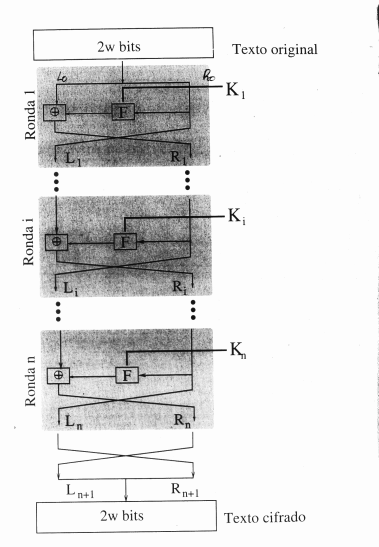
\includegraphics{RondasDES1.png}
 
 \newpage
 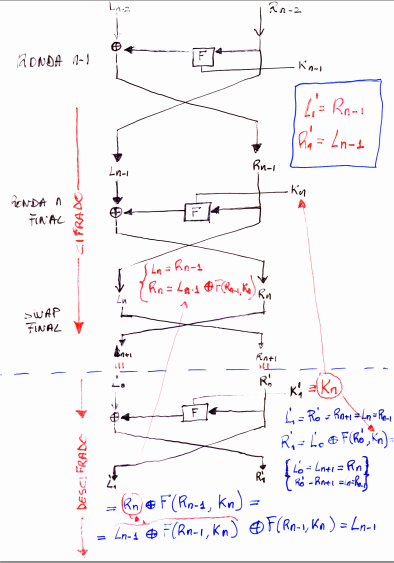
\includegraphics{RondasDES2.png}
 
 \newpage

\subsection{Principios de diseño de las S-Box en DES}

Esta sección también está muy bien explicada en el Stinson, p.79.

\begin{itemize}
	\item Las S no son lineales.
	$$f(x \oplus y) = f(x) \oplus f(y) + cte \implies \text{Esa constante es la que rompe la linealidad}$$
	
	\begin{example}
		\begin{center}
			\begin{tabular}{r  r  r  r  r  r }
				$b_1$ & $b_2$ & $b_3$ & $b_4$ & $b_5$ & $b_6$
			\end{tabular}
		\end{center}
		$$\downarrow$$
		$$\fbox{\textbf{     }S\textbf{     }}$$
		$$\downarrow$$
		\begin{center}
			\begin{tabular}{r  r  r  r }
				$c_1$ & $c_2$ & $c_3$ & $c_4$
			\end{tabular}
		\end{center}
		
		
	\end{example}
	
	\item \textbf{SAC} (Strict avalanch criterion)
	
	Este principio dice que la probabilidad de cambio debe estar equidistribuida.
	
	Esto es, que si cambio un bit de entrada, la probabilidad de que un bit de salida sea 0 o 1 es la misma.
	$$\forall i,j\text{  }P(c_i=1|\overline{b_j})  P(c_i=0|\overline{b_j}) = \frac{1}{2}$$
	Siendo $\overline{b_j}$ que he cambiado el bit $b_j$
	
	\item \textbf{BIC} (bit independence criterion)
	
	Busca que no haya dependencia entre los bits de salida (si cambia $c_3$, no condiciona a que cambie o no $c_2$) 
	$$\forall i,j,k \text{  } P(c_ic_j|\overline{b_k}) = P(c_i|\overline{b_k})\cdot P(c_j|\overline{b_k})$$
	
\end{itemize} 

\subsubsection{Métodos de construcción de las cajas S}
 \begin{itemize}
 	\item \textbf{Aleatorio}
 	\begin{itemize}
 		\item Aleatorio normal
 		\item Con comprobación
 	\end{itemize}
 	\item \textbf{Manual}: El DES utiliza este método
 	\item \textbf{Funciones Matemáticas}: El AES utiliza este método
 \end{itemize}
 
 \subsubsection{Propiedades del DES}
 \begin{itemize}
 	
 
 \item \textbf{Complementaria}: 
 
 Si $y = e_k(x)$ entonces $\overline{y} = e_{\overline{k}}(\overline{x})$.
 
 De esta forma el problema del ataque por texto escogido se reduce a la mitad.
 
 \item \textbf{Claves débiles}(de punto fijo):
 
  Son las claves que cumplen que: $$e_k(e_k(x))= x$$
 
 El DES tiene 4 claves débiles.
 
 \item \textbf{Claves semi-débiles}: 
 
 Son las claves que cumplen que: $$e_{k_1}(e_{k_2}(x)) = x$$
 El DES tiene 6 pares de claves semi-débiles.
 
 \item \textbf{Las claves en DES no forman un grupo}
 
 $$\nexists k_3 \text{ tal que } e_{k_3}(x) = e_{k_1}(e_{k_2}(x))$$
 
\end{itemize}

\subsubsection{Modos de operación del DES}

Hay varias formas de utilizar el DES. Vamos a ver algunas de ellas.

\begin{itemize}
	\item \textbf{ECB}(Electronic Code Book)
	
\end{itemize}
 % % Me faltan infinitas hojas % %
 
 $$D(x) = C(x) \text{ mod M(x)} \begin{cases}
 d_0 = a_0\cdot b_0 \oplus a_3 \cdot b_1 \oplus a_2 \cdot b_2 \oplus a_1 \cdot b_3 = C_0 \oplus C_4\\
 d_1 = a_1\cdot b_0 \oplus a_0 \cdot b_1 \oplus a_3 \cdot b_2 \oplus a_2 \cdot b_3 = C_1 \oplus C_5\\
 d_2 = a_2\cdot b_0 \oplus a_1 \cdot b_1 \oplus a_0 \cdot b_2 \oplus a_3 \cdot b_3 = C_2 \oplus C_6\\
 d_3 = a_3\cdot b_0 \oplus a_2 \cdot b_1 \oplus a_1 \cdot b_2 \oplus a_0 \cdot b_3 = C_3
 \end{cases}$$
 
 $$\left(\begin{matrix}
 d_0\\d_1\\d_2\\d_3
 \end{matrix} \right) = \left(\begin{matrix}
 a_0 & a_3 & a_2 & a_1\\
 a_1 & a_0 & a_3 & a_2\\
 a_2 & a_1 & a_0 & a_3\\
 a_3 & a_2 & a_1 & a_0\\
 \end{matrix}\right) \cdot \left( \begin{matrix}
 b_0\\
 b_1\\
 b_2\\
 b_3
 \end{matrix}\right)$$
 
 Esta operación esta definida  anivel de W (palabra).
 
 \section{Multiplicación por X}
 
 $$XTIME = x \cdot b(x) = b_3x^4 + b_2 x^3 + b_1 x^2 + b_0 x \textbf{ mod M(x)} = b_2x^3 +b_1x^2 + b_0x + b_3$$
 
 Vemos que esto lo que hace es un desplazamiento cíclico (rotación).
 
 $$XTIME(b_3 b_2 b_1 b_0) = b_2 b_1 b_0 b_3$$
 
 
 $$C(x) = x \cdot b(x) = \left(\begin{matrix}
 	C_0\\C_1\\C_2\\C_3
 \end{matrix} \right) = \left(\begin{matrix}
 00 & 00 & 00 & 01\\
 01 & 00 & 00 & 00\\
 00 & 01 & 00 & 00\\
 00 & 00 & 01 & 00\\
\end{matrix}\right) \cdot \left( \begin{matrix}
b_0\\
b_1\\
b_2\\
b_3
\end{matrix}\right)$$
 
 
\section{Diseños y criterios para el AES}

\subsubsection{Objetivos}

\begin{itemize}
	\item Resistente al C.D y C.L (criptoanálisis diferencial y lineal)
	\item Eficiente en varias plataformas
	
	Cumple este objetivo porque las operaciones son sumas, rotaciones y desplazamientos, que son operaciones que soporta cualquier plataforma informática. Y al ser de tan bajo nivel son my rápidas
	
	\item Código compacto y sencillo
	\item Fuerte base matemática
\end{itemize}

\subsubsection{Elementos de Diseño}

\begin{itemize}
	\item Capa lineal $\rightarrow$ Difusión
	\item Capa no lineal $\rightarrow$ Confusión
	
	Esto es antes de mezclarse la clave
	\item Capa de sumas de clave
	\item Clave variable $\rightarrow$ 128, 192, 256
	\item Bloque variable $\rightarrow$ 128, 192, 256
	
	El tamaño de bloque estándar es 128.
\end{itemize}

A pesar de utilizar los principios de confusión y difusión no es una esructura Feistel clásica.
 
\subsubsection{Diseño de Rijndael}

STATE (estado)

$$\overrightarrow{X} = x_0 , ...., x_n$$

$$x_i \in GF(2^8)|m(x)$$

Antes de estrar en el algoritmo se coloca este string en bloques para que el algoritmo pueda operar con él.

Se coloca de la siguiente forma:

Se pasa de esta notación:

	\begin{center}
		\begin{tabular}{l | l | c | r | r | r}
			$x_0$ & $x_4$ &  &  &  &  \\
			\hline
			$x_1$  & $x_5$ &  &  &  &  \\
			\hline
			$x_2$  &  &  &  &  &  \\
			\hline
			$x_3$ &  &  &  &  & $x_23$ \\
		\end{tabular}
	\end{center}
	
	$$\begin{cases}
	N_B = 4 \rightarrow 128\\
	N_B = 6 \rightarrow 192\\
	N_B = 8 \rightarrow 256\\
	\end{cases}$$

A esta notación	


	\begin{center}
		
		\begin{tabular}{l | c | r | r | r | r}
			$a_{00}$ & $a_{01}$ & $a_{02}$ & $a_{03}$ & $a_{04}$ & $a_{05}$\\
			\hline
			$a_{10}$ &   &   &   &   &  \\
			\hline
			$a_{20}$ &   &   &   &   &  \\
			\hline
			$a_{30}$ &   &   &   &   & $a_{35}$
			
		\end{tabular}
	\end{center}


\subsubsection{Tamaño de clave}

	\begin{center}
		
		\begin{tabular}{l | c | r | r }
		$K_{00}$ & $K_{01}$ & $K_{02}$ & $K_{03}$\\
		\hline
		$K_{10}$ &  &  & \\
		\hline
		$K_{20}$ &  &  & \\
		\hline
		$K_{30}$ &  &  & $K_{33}$
		
		\end{tabular}
	\end{center}
	
		$$\begin{cases}
		N_K = 4 \rightarrow 128\\
		N_K = 6 \rightarrow 192\\
		N_K = 8 \rightarrow 256\\
		\end{cases}$$
		
\subsubsection{Número de rondas}
	\begin{center}
		
		\begin{tabular}{l | c | r | r }
		$N_K$ & $N_B$ = 4 & $N_B$ = 6 & $N_B$ = 8\\
		\hline
		$N_K$ =4 &  10 & 12 & 14\\
		\hline
		$N_K$ = 6 & 12 & 12 & 14\\
		\hline
		$N_K$=8 & 14 & 14 & 14
		
		\end{tabular}
	\end{center}

\subsubsection{Una ronda AES}
\lstset{language=C, breaklines=true, basicstyle=\footnotesize}
\begin{lstlisting}[frame=single]

	Round(state , Subkey){
	
		ByteSub (STATE) ; //equivalente a S_Box, operaciones $GF(2^8)$, bit a bit
	
		ShiftRow(STATE); // desplazamiento de filas del STATE (operaciones W)
	
		MIXCOLUMN (STATE); // Operaciones con columnas utilizando W
	
		AddRoundKey (STATE, SubKey);
	} 
	
	+
	 
	FinalRound(S,SK){
		ByteSub(S);
		ShiftRow(S);
		AddRoundKey(S,SK);
	}
		
\end{lstlisting}

% -*- root: ../TIM.tex -*-
\section{Ejercicios}
\subsection{Hoja 1}
\begin{problem}[5]
Dada una sucesión $\lbrace f_n \rbrace \in R([a,b])$ que converge uniformemente a $f$, se pide demostrar que $f$ es integrable Riemann y que:
\[ \lim \int_{a}^{b} f_n = \int_{a}^{b} f \]

\solution
Supongamos que f es integrable Riemann, entonces tenemos que ver que:
\[ \forall \epsilon > 0 \ , \exists N \tq \forall n> N \ \abs{\int_a^b f_n - \int_a^b f} < \epsilon\]

Sabemos que:
\[\abs{\int_a^b f_n - \int_a^b f} \leq \abs{\int_a^b \abs{f_n -f}} dx\]

Recordemos la definición de convergencia uniforme

\begin{defn}[Convergencia\IS uniforme]
\[f_n \xrightarrow{uniforme} f \Leftrightarrow \forall \epsilon < 0, \exists N_{\epsilon} \tq \forall x \in [a,b]  \forall n \geq N_{\epsilon}, \abs{f_n (x) - f(x)} < \epsilon\]
\end{defn}

Si $n \geq N_{\frac{\epsilon}{b-a}}$ entonces, usando la definición de convergencia uniforme:

\[\int_a^b \abs{f_n(x) - f(x) dx} \leq \int_a^b \frac{\epsilon}{b-a}dx = \epsilon\]

Por tanto queda claro que si $f$ es integrable Riemann podemos conmutar el límite con la integral. Ahora queda ver por qué $f$ es integrable Riemann.

$f$ será integrable Riemann sii:
\[\forall \epsilon > 0 \ \exists P \tq \forall P' \prec P \]
\[\overline{J}_{P'}(f) - \underline{J}_{P'}(f) < \epsilon\]

Vamos a probarlo:
\[\overline{J}_P(f) - \underline{J}_P(f) = \sum(\sup_k f - \underset{k}{inf} f)\abs{I_k} \leq\]
\[\leq \sum\left( \abs{\sup_{k}f_n(x) - \sup_{k}f(x)} + \abs{\sup_{k}f_n(x) - \underset{k}{inf}f_n(x)} +  \abs{\underset{k}{inf}f_n(x) - \underset{k}{inf}f_n(x)} \right)\abs{I_k} \leq \]
Puesto que $f_n$ converge uniformemente a $f$ habrá un $n$ a partir del cual la distancia máxima entre $f_n$ y $f$ sea $\frac{\epsilon}{6}$ y por tanto la distancia máxima entre el supremo y el ínfimo de $f_n$ será menor que $\frac{\epsilon}{3}$
\[\leq \sum\left( \sup_{k} \abs{f_n(x) - f(x)} + \frac{\epsilon}{3} + \sup_k \abs{f_n(x) - f(x)} \right)\abs{I_k} \leq\]
Aplicando de nuevo la convergencia uniforme y tomando el máximo entre este $n$ y el calculado en el paso interior nos queda:
\[\leq \sum \left(\frac{\epsilon}{3} + \frac{\epsilon}{3} + \frac{\epsilon}{3} \right)\abs{I_k} = \sum\epsilon\abs{I_k}\]

Como hay convergencia uniforme entre $f_n$ y $f$ podemos hacer que los supremos sean tan pequeños como queramos y hacer así que el interior sumatorio quede menor que $\epsilon \abs{I_k}$

Puesto que $\epsilon$ es un número cualquiera podemos hacerlo tan pequeño como queramos haciendo que el último sumatorio escrito tienda a 0.

\end{problem}

\begin{problem}[6]

Sea $\lbrace f_n \rbrace$ una sucesión monótona creciente de funciones continuas en un intervalo $I=[a,b]$ que convergen en dicho intervalo a otra función continua $f$. Demuestra que entonces:
\[ lim \int_{a}^{b} f_n(x) = \int_{a}^{b} f(x) \]
\solution
Por ser funciones continuas son integrables Riemann. Si conseguimos demostrar que convergen uniformemente podemos emplear el ejercicio anterior y lo tendríamos hecho.
\end{problem}

\begin{problem}[7]
Dada la sucesión $I_k = (a_k, b_k)$ tales que $\bigcup_{k=1}^{N}~I_k~=~[a,b]$

Demostrar que:
\[b-a \leq \sum_{k=1}^N (b_k - a_k)\]

\solution
Vamos a utilizar la integral de Riemann como recomienda el ejercicio, utilizando la función indicatriz de cada intervalo $\ind_{I_k}$

Está claro que la función indicatriz del intervalo I es menor o igual que la suma de las funciones indicatrices de los intervalos. Lo cual es obvio, ya que si $x$ está en el intervalo, $x$ estará también en al menos uno de los intervalos $I_k$. Es decir:
\[\ind_{[a,b]} \leq \sum_{k=1}^{N} \ind_{I_k}\]

Utilizando la monotoneidad de la integral de Riemann podemos ``integrar a ambos lados'' obteniendo:

\[\int_{a}^{b} \ind_{[a,b]} \leq \int_{a_k}^{b_k} \sum_{k=1}^{N} \ind_{I_k}\]

Por la linealidad de la integral, podemos incluso meter la integral dentro del sumatorio
\[\int_{a}^{b} \ind_{[a,b]} \leq \sum_{k=1}^{N} \int_{a_k}^{b_k} \ind_{I_k}\]


Conociendo la integral de la función indicatriz tenemos el resultado de forma inmediata.
\[b-a \leq \sum_{k=1}^{N} ( b_k - a_k )\]

\end{problem}

\begin{problem}[9]
Dado $O\subset (a,b)$ unión numerable de intervalos disjuntos, se pide demostrar:
\[m^*(O)=\sum_{n=1}^{\infty} \abs{I_k}\]

\solution
Está claro que:
\[m^*(O) \leq \sum_{n=1}^{\infty} \abs{I_k}\]

Tenemos que demostrar la desigualdad contraria para poder concluir la igualdad.
Vamos a probar que:
\[m^*(O) \geq \sum_{n=1}^{\infty} \abs{I_k} - \epsilon\]

Puesto que sabemos que la suma infinita tiene un resultad finito (ya que $O$ es finito)
\[\forall \epsilon > 0 \exists N \tq \sum_{n=1}^N\abs{I_n} \geq \sum_{n=1}^{\infty} \abs{I_k} - \frac{\epsilon}{2}\]

Vamos a definir los intervalos $I'_n$ que serán un poco más pequeños que los $I_n$
\[\forall n=1,2,...,N \text{ definimos } I'_n=[a_n+\frac{\frac{\epsilon}{2}}{2^{n+1}}, b-\frac{\frac{\epsilon}{2}}{2^{n+1}}]\]

Ahora tenemos que:
\[\sum_{n=1}^N \abs{I'_n}=\sum_{n=1}^N\abs{I_n} - \frac{\epsilon}{2}\sum_{n=1}^{N}\frac{1}{2^n} \geq \sum_{n=1}^N\abs{I_n} - \frac{\epsilon}{2}\]

Definimos ahora el compacto:
\[K_n = \bigcup_{n=1}^N I'_n\]

Sean $J_n$ intervalos abiertos tales que $O \subset \bigcup_{n=1}^{\infty}J_n \Rightarrow K_n \subset \bigcup_{n=1}^{\infty}J_n$.

Por tanto
\[\exists N' \tq K_n \subset \bigcup_{n=1}^{N'}J_n=A_N\]

Vamos a fijarnos ahora en la medida exterior de $O$:

\[ m^*(O) = \inf\lbrace \sum_{n=1}^{\infty}\abs{J_n} \rbrace \geq \inf\lbrace \sum_{n=1}^{N'}\abs{J_n} \rbrace \geq \]
\[ \geq \inf\lbrace \int \ind_{A_N} \rbrace \geq \inf\lbrace \int \ind_{K_N} \rbrace \geq \inf\lbrace \sum_{n=1}^N\abs{I'_n} \rbrace \geq \]
\[ \geq \inf\lbrace \sum_{n=1}^N\abs{I_n} -\frac{\epsilon}{2}\rbrace \geq \inf\lbrace \sum_{n=1}^N\abs{I_n} -\epsilon \rbrace \]

Y obtenemos así la desigualdad buscada.
\end{problem}

\begin{problem}[10]
Dado un compacto K contenido en el intervalo (a,b), nos piden demostrar que:
\[m(K)<b-a\]

\solution
Consideremos la sucesión: $(a+\frac{1}{n}, b - \frac{1}{n})$, con $n >\frac{2}{b-a}$. Obviamente:
\[K \subset \bigcup_{n=n_0}^{\infty}(a+\frac{1}{n}, b - \frac{1}{n})\]

Como K es compacto:
\[\exists N \tq K \subset \bigcup_{n=n_0}^{N}(a+\frac{1}{n}, b - \frac{1}{n}) = (a+\frac{1}{N}, b - \frac{1}{N}) \]

Y llegamos a:
\[m(K) \leq b-a-\frac{2}{N} < b-a\]

\end{problem}

\begin{problem}[11]
Sea $C_n$ una sucesión creciente de subconjuntos medibles contenidos en (a,b) y sea $C$ la unión de estos subconjuntos. Se pide demostrar que:
\[m(C_n) \nearrow m(C)\]

\solution
Vamos a definir la sucesión $D_n$ como:
\[D_1=C_1 \ D_2 = C_2 \setminus D_1 \ D_3 = C_3 \setminus (C_1 \bigcup C_2) \ ...\]

Teniendo así C expresado como unión de los $D_n$, que son disjuntos. Así, la medida de $C$ queda expresada como:
\[m(C)=\sum_{n=1}^{\infty}m(D_n)\]
sabiendo que:
\[m(C_N)=\sum_{n=1}^{N}m(D_n)\]
\end{problem}

\begin{problem}[12]
Sea $C_n$ una sucesión decreciente de subconjuntos medibles contenidos en (a,b) y sea $C$ la intersección de estos subconjuntos. Se pide demostrar que:
\[m(C_n) \searrow m(C)\]
\solution

Tomando los complementarios, que también son medibles, tenemos una sucesión creciente de subconjuntos medibles contenidos en (a,b). Aplicando el ejercicio anterior llegamos a que:
\[(b-a)-m(C_n) \rightarrow (b-a)-m(C)\]
De donde puede deducirse que $m(C_n)$ decrece hacia $m(c)$.
\end{problem}

\begin{problem}[14]
Dada una sucesión $A_n$ contenida en (a,b), se pide demostrar que:
\[\lim_n m(A_0\Delta A_n)=0 \Rightarrow \lim_n m(A_n)=m(A_0) \]

Recordemos que:
\[ A_n \Delta A_0 = (A_n \setminus A_0) \cup (A_0 \setminus A_n) =
(A_n \cup A_0)\cap(A_n^c \cup A_0^c) \]
\solution
\[\lim_n m(A_0\Delta A_n)=0 \Rightarrow \lim_n m(A_0^c \cap A_n)=0 \wedge \lim_n m(A_0\cap A_n^c)=0\]

Escribimos ahora $A_n$ y $A_0$ como:
\[A_n = (A_n \cap A_0) \bigcup (A_n \cap A_0^c)\]
\[A_0 = (A_0 \cap A_n) \bigcup (A_0 \cap A_n^c)\]

De aquí podemos ver que:
\[m(A_n) = m(A_n \cap A_0) + m(A_n \cap A_n^c)\]
\[m(A_0) = m(A_0 \cap A_n) + m(A_0 \cap A_n^c)\]

Y restando llegamos a:
\[m(An) = m(A_0) -m(A_0 \cap A_n^c) + m(A_n \cap A_0^c)\]

Y sabemos que las medidas de estas intersecciones tienden a 0.
\end{problem}

\subsection{Hoja 2}
\begin{problem}[1]
Sea X=$\{a,b,c,d\}$. Comprueba que la familia de conjuntos
\[A = \{\emptyset, \{a\}, \{b\}, \{a,b\},\{c,d\},\{a,c,d\},\{b,c,d\}, \{a,b,c,d\}\}\]
forma una $\salgb$ en $X$.

\solution
\textcolor{blue}{Hecho por mi, no fiarse al 100\%}
Para comprobar que forma una $\salgb$ debemos comprobar que cumple las condiciones de $\salgb$:

\begin{enumerate}
\item \textbf{Debe contener al total y al vacío.}
Vemos que es cierto ya que contiene $\emptyset$ y $X=\{a,b,c,d,\}$.

\item \textbf{Debe ser cerrada por complementación}
Vemos que tomando cualquier elemento de $A$, su complementario respecto de $X$ también se contiene en $A$.

Los complementarios de los subconjuntos de un sólo elemento son los subconjuntos de tres elementos (y viceversa) y los dos subconjuntos de dos elementos son complementarios el uno del otro.

\item \textbf{Debe ser cerrada por uniones infinitas}
Puesto que el conjunto es finito no tiene sentido hablar de uniones infinitas, por lo que simplemente debemos comprobar que la unión de dos elementos cualesquiera de $A$ se contiene en $A$.

Fácilmente podemos observar que se cumple esta condición puesto que la unión de los subconjuntos de tres elementos con cualquier otro subconjunto nos da el total; la unión de uno de 2 elementos y uno de 2 nos da uno de los de 3; la unión de los de 2 elementos da el total y la unión de los de 1 elemento nos da uno de 2 elementos.
\end{enumerate}

\end{problem}
\begin{problem}[2]
Sea $X=\{a,b,c,d\}$. Se pide construir la $\salgb$ generada por $\algb{E}=\{\{a\},\{b\}\}$ y por $\algb{E}=\{\{a\}\}$

\solution
Sabemos que en un conjunto finito toda álgebra es una $\salgb$, ya que la diferencia entre álgebra y $\salgb$ era el cierre por uniones infinitas numerables. Si un conjunto es finito, $\algb{P}(X)$ será finito y no habrá posibilidad de hacer uniones infinitas.

Vamos a construir la mínima álgebra que contiene a $\algb{E}$ a pelo, forzando que se cumplan las propiedades de un álgebra de conjuntos:
\[\algbM(\{\{a\}\}) = \{\emptyset, \{a\}, \{b,c,d\}, \{a,b,c,d\}\}\]
\[\algb{M}(\{\{a\},\{b\}\})=\{\emptyset, X, \{a\}, \{b\}, \{a,b\}, \{b,c,d\}, \{a,c,d\}, \{c,d\}\}\]

\obs Si tomamos $A_1=\{a\} \ y \ A_2 = \{b\}$ podemos comprobar fácilmente que:
\[\algb{M}(A_1 \cup A_2) \neq \algb{M}(A_1) \cup \algb{M}(A_2)\]
\end{problem}

\begin{problem}
Comprobar que la unión de dos $\salgb$ no tiene por qué ser una $\salgb$. Poner un ejemplo en el que las $\salgb$ de partida tengan infinitos elementos.

\solution
\textcolor{blue}{Hecho por mi, no fiarse al 100\%}

Para comprobarlo podemos apoyarnos en el ejemplo anterior y ver que
\[\algb{M}(A_1) \cup \algb{M}(A_2) = \{\emptyset, \{a\}, \{b\}, \{b,c,d\}, \{a,c,d\}, \{a,b,c,d\}\}\]
es unión de dos $\salgb$ pero no es $\salgb$ ya que $\{a\} \cup \{b\} = \{a,b\} \notin \algbM$

Vamos ahora a buscar un ejemplo de $\salgb$ de infinitos elementos, como pide el enunciado: si tomamos el álgebra formada por los pares (E) y la formada por los impares (O), su unión no es álgebra: eg \{1,2\} $\notin$ E $\cup$ O.
\end{problem}

\begin{problem}[4]
Dada una función $\appl{g}{X}{Y}$ y sea $\algb{A}$ una $\salgb$ de X, demostrar que:
\[\algb{B}=\{E\subset Y \tq g^{-1}(E)\in \algb{A}\}\]
es una $\salgb$

\solution
Debemos comprobar que $\algbB$ cumple las condiciones de $\salgb$. Para ello basta con ver que se cumplen las siguientes dos propiedades sobre $g$
\begin{enumerate}
\item
\[g^{-1}(E_1 \cup E_2)=g^{-1}(E_1) \cup g^{-1}(E_2)\]
\item
\[g^{-1}(Y \setminus E) = X - g^{-1}(E)\]
\end{enumerate}
Vamos a comprobarlas pues
\begin{proof}
\begin{enumerate}
\item
\[x\in g^{-1}(E_1 \cup E_2) \iff g(x) \in E_1 \cup E_2 \iff  \exists i=1,2 \ g(x) \in E_i \iff \]
\[\iff \exists i=1,2 \ x\in g^{-1}(E_i) \iff x\in g^{-1}(E_1) \cup g^{-1}(E_2) \]
\item
\[x\in g^{-1}(Y \setminus E) \iff g(x) \in Y \setminus E \iff g(x) \notin E \iff x \notin g^{-1}(E) \iff x \in X\setminus g^{-1}(E)\]
\end{enumerate}

\end{proof}
Así, por la primera propiedad queda claro que $\algb{B}$ es cerrado por uniones y con la segunda propiedad vemos que es cerrado por complementación. Es decir:
\[\{E_i\}_{i_1}^{\infty} \in \algb{B} \implies \bigcup_{i=1}^{\infty} E_i \in \algb{B}\]
ya que $g^{-1}(\bigcup_{i=1}^{\infty} E_i) = \bigcup_{i=1}^{\infty} g^{-1}(E_i) \in A$

Podemos hacer lo mismo para ver el cierre por complementación

Además, queda claro que tanto el vacío como el total se contienen en $\algb{B}$, ya que $X$ y $\emptyset \in A \implies g^{-1}(Y)=X \in A, g^{-1}(\emptyset)=\emptyset \in A \implies Y, \emptyset \in \algb{B}$ por lo que se trata de una $\salgb$
\end{problem}

\begin{problem}[5]
Dada una función $\appl{g}{X}{Y}$ y sea $\algb{B}$ una $\salgb$ de Y, demostrar que:
\[\algb{A}=\{g^{-1}(E) \tq E \in \algb{B}\}\]
es una $\salgb$

\solution
Vamos a comprobar las propiedades de cierre por unión y por complementación:
\begin{enumerate}
\item. Debemos ver que:
\[A_1, A_2\in \algb{A} \Rightarrow A_1 \cup A_2 \in A\]
Lo cual es cierto ya que, como demostramos en el ejercicio anterior:
\[g^{-1}(E_1 \cup E_2)=g^{-1}(E_1) \cup g^{-1}(E_2)\]
Si tomamos $A_i=g^{-1}(E_i)$ queda claro que:
\[A_1 \cup A_2 = g^{-1}(E_1) \cup g^{-1}(E_2) = g^{-1}(E_1\cup E_2) \Rightarrow g^{-1}(E)\]
para algún $E\in \algb{B}$ por ser esta una $\salgb$.

\item Ahora tenemos que ver que:
\[A \in \algb{A} \Rightarrow X\setminus A \in \algb{A}\]
Con la segunda propiedad del ejercicio anterior queda claro que es cierto
\end{enumerate}

Por tanto, $\algb{A}$ cumple todas las propiedades de $\salgb$.

\obs En este caso resultaba obvio ver que $\algbA$ contenía al vacío y al total por lo que ni nos hemos molestado. Si no estuviese tan claro habría que comprobarlo al igual que las otras propiedades.

\end{problem}

\begin{problem}[4-5Bis]
\textbf{Inventado por el profesor.}

Vamos a ver que la imagen directa de una $\salgb$ no tiene por qué ser una $\salgb$, es decir:
dada una función $\appl{f}{X}{Y}$ y sea $\algb{A}$ una $\salgb$ de X, demostrar que:
\[\algb{B}=\{g(E) \tq E \in \algb{A}\}\]
no es necesariamente una $\salgb$

\solution
Esto es sencillo puesto que si la función $f$ no es suprayectiva, entonces $Y \neq g(E)$ para cualquier $E$, por lo que $\algb{B}$ no contiene al total y, por tanto no sería $\salgb$.

Supongamos ahora que  la función $f$ es suprayectiva. En este caso seguiríamos teniendo problemas si $f$ no es inyectiva.

Tomemos por ejemplo $g(x)=x^2$. En este caso, $g((-\infty, 0] \cup [0, \infty))=g(0)=0 \neq g((-\infty, 0]) \cup g([0, \infty))$.
\end{problem}

\begin{problem}[6]
Demuestra que una álgebra $\algb{A}$ es una $\salgb$ si y sólo si es cerrada para uniones numerables crecientes.

\solution
Vamos a demostrar las dos direcciones de la implicación:
\begin{itemize}
\item $\Rightarrow$
Es obvio ya que una $\salgb$ es un álgebra cerrada por uniones numerables y por tanto, es cerrada para el caso concreto de uniones numerables crecientes.
\item $\Leftarrow$

Dado un conjunto $\{A_i\}_{i=1}^{\infty}$ tal que $A_i \in \algb{A} \quad \forall i$, construyo otro de la siguiente forma:
\[B_n = \bigcup_{i=1}^{n} A_i\]
de tal forma que $B_i \subset B_j \quad \forall i<j$.

Ahora, por hipótesis, sabemos que la unión de los $B_i$ se contiene en la $\salgb$, luego:
\[\bigcup_{n=1}^{\infty} A_i=\bigcup_{n=1}^{\infty} B_i \in \algb{A}\]\qed

\end{itemize}
\end{problem}

\begin{problem}[7]
Determina el álgebra $\algb{A}$ generada por la colección de los subconjuntos finitos de un conjunto X no-numerable. Determina la $\salgb$ generada por $\algb{A}$. Estudiar el mismo problema en caso de que el conjunto X sea infinito numerable

\solution
Dado el conjunto de todos los subconjuntos finitos, para convertirlo en una $\salgb$ debemos asegurarnos de que sea cerrado por uniones numerables y por complementación.

Para hacerlo cerrado por uniones numerables, debemos incluir todos los conjuntos numerables, ya que cualquiera de estos puede obtenerse como unión de conjuntos finitos.

Además, si queremos que sea cerrado por complementación, tendremos que incluir los complementarios de todos los conjuntos mencionados anteriormente, es decir, debemos incluir todos aquellos conjuntos cuyo complementario sea numerable.

Así, vamos a construir de forma directa la $\salgb$ pedida:
\[\algb{M}(\algb{E})=\{ E\subset X \tq E \text{ numerable o finito, } E^c \text{ numerable o finito}\}\]

Podemos comprobar fácilmente que es una $\salgb$ observando que cumple las propiedades necesarias siguiendo el mismo razonamiento que el realizado para construirla (la unión de numerables o finitos sigue siendo numerable o finita y su complementario cumple la propiedad de tener complementario numerable o finito).

Es la mínima por construcción.

Si X es infinito numerable entonces
\[\algb{M}(\algb{E})=\algb{P}(X)\]
aplicando la misma regla de construcción, ya que todos los subconjuntos de $\algb{P}(X)$ son numerables.
\end{problem}

\begin{problem}[8]
La $\salgb$ de (0,1] engendrada por:
\[\algb{E}= \{(0, \frac{1}{n}]: n=1,2,...\}\]
está formada por uniones finitas o numerables de intervalos (a,b]. Estudia cómo son estos intervalos.

\solution
Queremos ver como son los intervalos (a,b] tales que:
\[\algb{M}(\algb{E})=\bigcup_{i=1}^{\infty}\{(a_i, b_i]\}\]

Vamos a ver cuáles son los elementos que tenemos en $\algb{M}(\algb{E})$. Aquí, además de los propios elementos de $\algb{E}$ tenemos:
\begin{itemize}
\item \textbf{Complementarios} Son de la forma $(\frac{1}{n}, 1]$

\item \textbf{Intersecciones} Son de la forma $(\frac{1}{m}, \frac{1}{n}]$ con m>n

\item \textbf{Uniones} Uniendo dos elementos seguimos estando en $\algb{E}$, así que no ganamos nada nuevo.
\end{itemize}

Puesto que las uniones contienen a los complementarios, tenemos que los intervalos que forman la $\salgb$ son de la forma:
\[\algb{M}(\algb{E})=\bigcup_{i=1}^{\infty}\{(a_i, b_i]: a_i =\frac{1}{m}, \ b_i = \frac{1}{n} \ m>n\}\]
\end{problem}

\begin{problem}[9]
Describe la $\salgb$ generada por:
\[\algb{E}= \{N \subset \nat \tq \forall n \in \nat, \ 2n \in N\}\]

\solution
\textcolor{blue}{Hecho por mi. No fiarse al 100\%}

Vemos que el conjunto $\algb{E}$ está formado por todos los conjuntos que contienen a todos los pares.

Esta claro que la unión y la intersección de conjuntos de $\algb{E}$ pertenecen a $\algb{E}$ ya que contendrán a todos los pares.

Los complementarios serán los subconjuntos de $\nat$ que sólo contengan números impares.

Si combinamos todos estos conjuntos formaremos la mínima $\salgb$ que lo contenga todo. Es decir:
\[\algb{M}(\algb{E})=\{N \subset \nat \tq \text{N no contiene ningún par, o N contiene a todos los pares}\}\]
\end{problem}

\begin{problem}[10]
Sea $\algb{M}$ una $\salgb$ de cardinal infinito. Demuestra que tiene cardinal no numerable.
\solution
Si la $\salgb$ es infinita podemos encontrar una colección numerable y disjunta de elementos de la misma. (Lo podemos hacer tomando una colección numerable y haciéndola disjunta mediante la eliminación en cada elemento de la unión de los anteriores).

Denotamos a esta colección como: $\{A_n:n\in \nat\}$.

Ahora vamos a construir una colección infinita de $A_x$ como sigue:
\[\forall x \in (0,1) \text{ obtenemos el desarrollo en base 2 de } x=0,x_1,x_2,x_3,...\]
\[A_x=\bigcup_{n=1}^{\infty}A'_n \text{ donde } A'_n=\left\{ \begin{array}{lcc}
             A_n &   si  & x_n = 1 \\
             \\ \emptyset &  si  & x_n \neq 1
             \end{array}
   \right.\]

Como no puede darse el caso de dos $A_x$ iguales, es necesario tomarlos todos para construir $\algb{M}$ y puesto que el número de $A_x$ es no numerable (uno por cada real en el intervalo (0,1)), tenemos que el número de elementos de $\algb{M}$ es no numerable.

\end{problem}

\begin{problem}[11]
Hallar una cota superior al número de elementos que puede tener una $\salgb$ $\algb{M}$ generada a partir de un conjunto con n elementos:
\solution
El enunciado nos dice que tenemos un conjunto $ε\subset \algb{P}(X) \tq ε=\{A_1,...A_n\}$

Si el conjunto ε es una partición del conjunto $X$ (división de $X$ en subconjuntos disjuntos dos a dos), entonces la mínima $\salgb$ generada tendrá $2^{\#ε}$ elementos.
\begin{proof}
Vamos a considerar todas las posibles uniones de los elementos de ε, que deberán pertenecer a $\algb{M}(ε)$.
Para poder contar estas uniones, vamos a representar cada unión mediante un número binario de longitud \# ε, donde los 1s nos indican qué elementos de ε estamos considerando.

Queda claro así que el conjunto de todas las uniones posibles tiene $2^{\# ε}$ elementos. Estas uniones serán todas disjuntas puesto que así lo son los elementos que las generan. Además, esto implica que las intersecciones son vacías y el complementario de cada elemento está formado por la unión del resto y, por lo tanto, también se contiene en el conjunto de uniones.

Obviamente esta construcción genera la mínima $\salgb$ generada por el conjunto ε y que tiene el cardinal buscado.
\end{proof}

Pero el caso que nos concierne es ligeramente distinto, pues no son disjuntos.

Si tomamos el primer elemento, podemos construir una partición de $X$ a partir de él, considerando los conjuntos: $A_1 \ A_1^c$.

Cogiendo ahora un segundo conjunto $A_2 \in ε$, tenemos entonces que los cuatro conjuntos: $A_1 \cap A_2, \ A_1^c \cap A_2 \ A_1^c \cap A_2^c \ A_1 \cap A_2^c$, se contendrían en la $\salgb$. Estos cuatro conjuntos podrían ser distintos todos ellos, o podrían coincidir. Como mucho darán cuatro conjuntos distintos y como poco 2.

\textbf{Recordemos que la un álgebra (y por tanto una $\salgb$) es cerrada por intersecciones ya que:}
\[A_1, A_2 \in \algb{A} \implies A_1 \cap A_2 = (A_1^c\cup A_2^c)^c \in \algb{A}\]

Para dejarlo claro, los hemos conseguido considerando las posibles intersecciones del segundo conjunto que hemos cogido y su complementario con los conjuntos que teníamos en el paso anterior.

Tomo ahora un tercer elemento de ε distinto de los anteriores, y construyo todas las combinaciones posibles con los 4 elementos anteriores, de forma similar a como construimos esas mismas combinaciones, siendo $A_1$ cada una de esas intersecciones y $A_2$ nuestro tercer conjunto.

En cada paso tenemos $2^i$ conjuntos disjuntos dos a dos que constituyen una partición de $X$. Cuando lleguemos al final, tendremos la partición que contiene a todos los elementos de ε.

Es decir, tenemos $N=2^n$ elementos (o menos) disjuntos que generan nuestra $\salgb$.

Puesto que ahora tenemos un ε como el que comentamos al inicio del ejercicio, tenemos que:
\[\#\algb{M}(ε)=2^N\]
\end{problem}

\begin{problem}[12]
Se llama $\sigma$-anillo de subconjuntos de un conjunto $X$ a toda familia no vacía $\algb{F}$ de subconjuntos de $X$ cerrada para uniones numerables y para las diferencias. Demuestra que todo $\sigma$-anillo es también cerrado para intersecciones numerables. Demuestra que todos $\sigma$-anillo de $X$ es una $\salgb \iff X \in \algb{F}$
\solution
Vamos a probar que un $\sigma$-anillo es cerrado para intersecciones numerables.
Dada una familia infinita numerable $A_i \in \algb{F}$ sabemos que $\bigcup A_i \in \algb{F}$ y lo denotamos por $A$.
Entonces:
\[A \setminus \bigcap A_i = \bigcup(A\setminus A_i) \in \algb{F} \Rightarrow A\setminus (A \setminus \bigcap A_i)=\bigcap A_i \in \algb{F}\]

La condición que le falta a un $\sigma$-anillo para ser una $\salgb$ es contener al total. Por tanto, si añadimos el total ya estamos forzando el cumplimiento de la última condición.
\end{problem}

\begin{problem}[13]
Se llama ``clase monótona'' de un conjunto $X$ a toda familia no vacía $\algb{M}$ de subconjuntos de $X$ que sea cerrada para las uniones crecientes y para las intersecciones decrecientes (es decir, si $\forall i=1,2,.. \ C_i \in \algb{M}$ y $C_i \subset C_{i+1}$ o $C_i \supset C_{i+1}$ entonces $\cup_iC_i \in \algb{M}$ o $\cap_iC_i \in \algb{M}$, respectivamente).

Demuestra que toda $\salgb$ es clase monótona. Da un ejemplo de una clase monótona que no sea $\salgb$
\solution

\begin{defn}[Clase monótona]
$\algb{M} \subset \algb{P}(X)$ es clase monótona si para toda sucesión $\{A_i\}$ de elementos de $\algb{M}$ se cumple que:
\begin{enumerate}
\item \[\forall i A_i \subset A_{i+1} \Rightarrow \bigcup_{n=1}^{\infty}A_i \in \algb{M}\]
\item \[\forall i A_i \supset A_{i+1} \Rightarrow \bigcap_{n=1}^{\infty}A_i \in \algb{M}\]
\end{enumerate}
\end{defn}
Basta con que probemos la primera propiedad ya que la segunda sale por complementación.

Es obvio que toda $\salgb$ es clase monótona, puesto que una $\salgb$ es cerrada para uniones numerables y, en concreto, lo será para uniones numerables crecientes.

La parte interesante del ejercicio es la que sigue.

Vamos a buscar el ejemplo de clase monótona que no sea $\salgb$.
Para el ejemplo basta con encontrar una cadena finita de conjuntos crecientes lo que nos garantiza el cumplimiento de las propiedades de una clase monótona, pero dista mucho de ser una $\salgb$.

Un ejemplo concreto sería:
\[\nat \supset \{2n, \ \forall n \in \nat\}\supset \{4n, \ \forall n \in \nat\}\supset \{8n, \ \forall n \in \nat\}\supset \{16n, \ \forall n \in \nat\}\supset \emptyset\]
La clase monótona sería una subclase de $\algb{P}(\nat)$ formada por todos los conjuntos aquí descritos y no es una $\salgb$, ya que no es cerrada por complementación.
\end{problem}

\begin{problem}[14]
Demuestra que la mínima clase monótona que contiene un álgebra dada $\algb{A}$ es también una $\salgb$

\solution
\textcolor{blue}{Atención, ejercicio clave}
\begin{center}
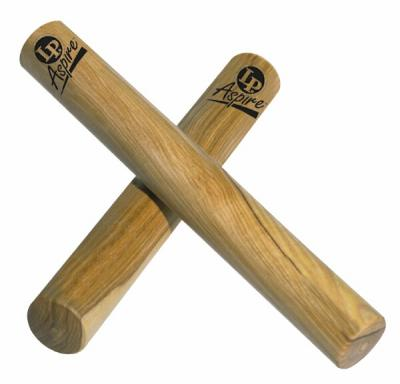
\includegraphics[scale=0.5]{img/clave.jpg}
\end{center}

Vamos a observar dos cosas:
\begin{enumerate}
\item Existe al menos una clase monótona que contiene a un conjunto $\algb{E}$, que es $\algb{P}(X)$
\item La intersección de clases monótonas es clase monótona. Demostración trivial.
\end{enumerate}

Tras estas observaciones podemos hablar de la mínima clase monótona que contiene a $\algb{E}$ como la intersección de todas las clases monótonas que lo contienen y sabemos que la intersección no es vacía por que hay al menos una.

Vamos a tener que hacer dos observaciones más:
\begin{enumerate}
\item Si una clase de conjuntos es álgebra y clase monótona, entonces es $\salgb$.
\item Sea $\algb{A}$ es un álgebra y $\algb{C}$ la mínima clase monótona que contiene a $\algb{A}$, entonces $\algb{C}$ es un álgebra.
\end{enumerate}

%\textcolor{red}{Hecho por mi. No fiarse al 100\%}
% Rehecho en clase y corregidos errores
\begin{proof}
\begin{enumerate}
\item Si nos apoyamos en el ejercicio 6, vemos clara esta demostración. Por ser clase monótona será cerrada para uniones numerables crecientes. Apoyándonos en el ejercicio 6, tenemos que un álgebra cerrada por uniones crecientes numerables es una $\salgb$

\item Vamos a ver que decir que un conjunto $\algb{C}$ es un álgebra es equivalente a decir:
\[\forall E,F \in \algb{C}, E\cap F, \ E\setminus F, \ F\setminus E \in \algb{C}\]

Vamos a definir:
\[\forall E \in \algb{C}, \ \algb{C}(E)=\{F \in \algb{C}: \  E\cap F, \ E\setminus F, \ F\setminus E \in \algb{C}\} \]

Vamos a comprobar que $\algb{C}(E)$ es una clase monótona comprobando las dos propiedades que definen una clase monótona:
\begin{itemize}
\item Dada una sucesión de conjuntos $\{F_i\} \in \algb{C}(E)$ tales que $F_i \subset F_{i+1}$ vemos que:
\ppart \[(\cup F_i)\setminus E = \cup (F_i \setminus E) \in \algb{C}\]
\ppart \[E \setminus (\cup F_i) = \cap(E \setminus F_i) \in \algb{C}\]
\ppart \[E \cap (\cup F_i) = \cup (E \cap F_i) \in \algb{C}\]

De donde podemos deducir que
\[F_i \in \algb{C}\]

\item Tomemos ahora una sucesión de conjuntos $\{F_i\}\in \algb{C}(E)$ tales que $F_i \supset F_{i+1}$ vemos que:
\ppart \[(\cap F_i)\setminus E = \cap (F_i \setminus E) \in \algb{C}\]
\ppart \[E \setminus (\cap F_i) = \cup(E\setminus F_i) \in \algb{C}\]
\ppart \[E \cap (\cap F_i) = \cap (E \cap F_i)\in \algb{C}\]

De donde podemos deducir que, en este caso:
\[F_i \in \algb{C}\]
\end{itemize}

Además esta claro que:
\[\forall E,F \in \algb{C}, \quad E\in \algb{C}(F) \iff F \in \algb{C}(E)\]

Vamos a ver ahora que $\algb{C} \subset \algb{C}(E) \quad \forall E \in \algb{A}$

Para probarlo, basta con ver que $\forall E \in \algb{A}, \ \algb{C}(E)$ es monótona, $\algb{A} \subseteq \algb{C}(E)$ y que $\algb{C}$ es la mínima clase monótona que contiene a $\algb{A} \implies \algb{C} \subseteq \algb{C}(E) $.

\end{enumerate}
\end{proof}
\end{problem}

\subsection{Hoja 3}
A lo largo de esta hoja se piden realizar varias demostraciones. La terminología que ha establecido Patricio en estos ejercicios consiste en llamar comprobaciones a los ejercicios mas triviales, pruebas a los del un nivel intermedio y demostraciones a los que realmente requieren esfuerzo.

\begin{problem}
Sea $(X, \algbM, µ)$ un espacio de medida. Si $E,F \in \algbM$ comprueba que
\[µ(E)+µ(F)=µ(E\cup F) + µ (E\cap F)\]

\solution
En el enunciado pide comprobar por lo que, según Patricio, debe ser bastante trivial.

En este caso tiene razón, ya que lo ocurre es conceptualmente muy sencillo. Al sumar $µ(E)+µ(F)$ la intersección la estoy teniendo en cuenta dos veces (una al medir $E$ y otra al medir $F$).

Para escribir una demostración formal observemos que:
\[E \cup F = (E \setminus F) \cup (F\setminus E) \cup (E \cap F)\]
Puesto que se trata de una unión disjunta, y µ es una medida, si tomamos la medida de todo ello obtenemos:
\[µ(E \cup F) = µ(E \setminus F) + µ(F\setminus E) + µ(E \cap F) = µ(E)-µ(F\cap E)+µ(F)-µ(E \cap F)+µ(E \cap F) =\]
\[= µ(E) + µ (F) +µ (E \cap F)\]
\end{problem}

\begin{problem}
Sea $(X, \algbM, µ)$ un espacio de medida y sea $E \in \algbM$. Para cada $A \in \algbM$ sea $µ_E(A)=µ(E\cap A)$.

Comprueba que $µ_E$ es una medida en $\algbM$
\solution
Si recordamos la definición de medida en un espacio medible, vemos que se trata de una aplicación de los subconjuntos del espacio a los reales que cumple dos propiedades básicas:
\begin{enumerate}
\item La medida del vacío es 0
\item La medida de una unión de conjuntos disjuntos es la suma de las medidas de cada uno de los conjuntos
\end{enumerate}

Si queremos probar que $µ_E$ es una medida deberemos comprobar que se satisfacen esas dos condiciones, es decir:
\[µ_E(\emptyset) = 0\]
\[µ_E(\bigcup A_n) = \sum µ_E(A_n)\]

La primera propiedad es trivial, ya que, por ser µ una medida tenemos:
\[µ_E(\emptyset)=µ(E \cap \emptyset)=µ(\emptyset)=0\]

Para la segunda propiedad vemos que:
\[µ_E(\bigcup A_n)=µ(E \cap (\bigcup A_n)) = µ(\bigcup(A_n \cap E)) \text{ con } A_i\cap A_j = \emptyset \ \forall i\neq j\]
Puesto que los $A_n \cap E$ son disjuntos y $µ$ es una medida sobre $\algbM$ tenemos que:
\[µ(\bigcup(A_n \cap E))=\sum µ(E \cap A_n) = \sum µ_E(A_n)\]

\end{problem}

\begin{problem}
\begin{enumerate}
\item Comprueba que una medida $\sfin$ es semifinita
\item Sea $X$ un conjunto no numerable y sea µ la medida discreta en $(X, \algbP (X))$, comprueba que µ es  semifinita pero no $\sfin$
\end{enumerate}

\solution
\begin{enumerate}
\item
Sabemos que, por definición de $\sfin$, el conjunto $X$ (sobre el que está definida la medida) puede expresarse como una unión de elementos de la $\salgb$ de medida finita. Es decir:
\[\exists \{E_n\}_{n \in \nat} \subset \algbM \tq X = \bigcup E_n \text{ con } µ(E_n)< \infty \forall n\]

Y para ver que µ es semifinita, por definición, debemos ver que todo subconjunto $E$ de la $\salgb$ tiene un subconjunto contenido también en la $\salgb$ de medida finita. Es decir:
\[\forall E \subset \algbM \text{ con } µ(E)>0, \ \exists A \in \algbM \text{ con } A\neq \emptyset \ A \subset E \text{ y } 0<µ(A) < \infty\]

Puesto que $X$ puede expresarse como unión de los $E_n$ está claro que:
\[E= \bigcup (E \cap E_n)\]
y puesto que no podemos garantizar que sean disjuntos los elementos de la unión tenemos:
\[µ(E)=µ(\bigcup (E \cap E_n))\leq \sum(µ(E \cap E_n))\]

Entonces
%TODO WTF?
\[\exists n \tq 0<µ(E \cap E_n) < \infty\]
Y basta con tomar $A=E \cap E_n \subset E$

\item
Recordemos que la medida discreta es la que, aplicada sobre un conjunto, nos devuelve el cardinal del conjunto si este es finito o infinito en caso contrario.

Para ver que es semifinita nos fijamos en que
\[µ(E) > 0 \implies E \neq \emptyset \implies \exists a \in E\]
En ese caso
\[\{a\}\subset E \text{ con } µ(\{a\})=1\]
Por lo que es semifinita
%TODO WTF?

Ahora vamos a comprobar que no es $\sfin$ por reducción al absurdo.

Si fuese $\sfin$,
\[\exists \{E_n\}_{n \in \nat} \subset \algbM \tq X = \bigcup E_n \text{ con } µ(E_n)< \infty \forall n\]
es decir, el cardinal de $E_n$ sería finito  y $X= \bigcup_{n \in \nat }E_n$ lo que implicaría que $X$ es numerable, en contradicción la hipótesis inicial.

\end{enumerate}
\end{problem}

\begin{problem}
Sea $X$ un conjunto infinito numerable, para $A \subset X$ se define
\[µ(A)=\left\{ \begin{array}{lcc}
             0 &   si  & A \text{ es finito} \\
             \\ \infty &  si  & A \text{ es infinito}
             \end{array}
   \right.\]

\begin{enumerate}
\item Comprueba que µ es finitamente aditiva (en $(X, \algbP (X))$) pero no numerable aditiva
\item Comprueba que existe una sucesión creciente de conjuntos $\{A_n\}$ tal que:
\[\forall n \in \nat, \ µ(A_n)=0 \ y \ \lim_{n} A_n =X\]
\end{enumerate}
\solution
\begin{enumerate}
\item Comprobar que es numerablemente aditiva implica comprobar que la medida de la unión de conjuntos disjuntos es la suma de las medidas.

Vamos a comprobarlo por casos:
Tomemos una sucesión finita y disjunta de $A_n$.
\begin{enumerate}
\item Si todos son finitos las medidas serán 0, la unión será finita y también tendrá medida 0.

\item Si al menos uno es infinito, entonces la medida sería infinita y la suma de medidas será infinito también.

\item Sin embargo, si tomo una sucesión numerable de conjuntos finitos, la medida de cada uno de ellos sería 0 pero la unión sería infinita por lo que tendría medida infinita.

Para obtener elegantemente estos conjuntos podemos tomar una numeración de los elementos de X (ya que es numerable). Es decir, consideramos:
\[X= \bigcup_{n=0}^{\infty}A_n \text{ donde } A_n=\{a_n\}\subset X\]
En este caso µ(X) es infinita pero a la izquierda tendríamos una suma de 0s ($µ(A_n)$) que nos daría 0
\end{enumerate}
Queda claro que es finitamente aditiva pero no numerablemente.

\item Vamos a definir la sucesión creciente:
\[A_n = \bigcup_{i=0}^{n}\{a_n\} \ a_n \in X\]
Puesto que cada $A_n$ será finito, tendrá medida 0 y la sucesión converge a $X$
\end{enumerate}

\end{problem}

\begin{problem} Sean $(X, \algbM, μ)$ un espacio de medida y $\{A_n\}_{n∈ℕ}$ una sucesión de conjuntos medibles. Si $A= \bigcup_{j=0}^∞ A_j$, prueba que \[ μ(A) = \lim_{n\to∞} μ\left(\bigcup_{j=0}^n A_j\right)\]
\solution

Vamos a demostrarlo viendo primero que \[ μ(A) ≥ \lim_{n\to∞} μ\left(\bigcup_{j=0}^n A_j\right) \] y es que es fácil ver que $\bigcup_{j=0}^n A_j ⊆ A \; ∀n$, luego \[ μ(A) ≥ μ\left(\bigcup_{j=0}^n A_j\right)\quad ∀n \]

Ahora bien, ¿puede ser esa desigualdad estrictamente mayor cuando $n\to∞$? Si lo fuera,
\[ μ(A) > μ\left(\bigcup_{j=0}^∞ A_j\right) \]
entonces $\bigcup_{j=0}^∞ A_j \subsetneq A$, lo que implica una contradicción.
\end{problem}

\begin{problem}[6]
Sea ($X, \algbM, µ$) un espacio de medida y $\{E_n\} $ una sucesión de conjuntos en $\algbM$. Demuestra que si existe un k tal que $µ(\bigcup_{i=k}^{\infty}E_i) < \infty$ entonces:
\[µ(\liminf (E_j))<\liminf (µ(E_j)))\]
\[µ(\limsup (E_j))>\limsup (µ(E_j)))\]

En particular si µ(X) < $\infty$ entonces:
\begin{enumerate}
\item
\[µ(\liminf E_j) \leq \liminf µ(E_j) \leq \limsup µ(E_j) \leq µ(\limsup(E_j))\]
\item Si existe $\lim E_j$ entonces $µ(\lim E_j)=\lim µ(E_j)$.
\end{enumerate}
Indica en qué punto es necesaria la condición $µ(\bigcup_{j=k}^{\infty}E_j)< \infty$ para al menos un k.
\solution
Recordemos algunas 'definiciones' necesarias para resolver el ejercicio:
\[\liminf (E_k) = \bigcup_{j=0}^{\infty} \bigcap_{k=j}^{\infty} E_k\]
\[\limsup (E_k)= \bigcap_{j=0}^{\infty} \bigcup_{k=j}^{\infty} E_k\]
Basándonos en la \href{http://en.wikipedia.org/wiki/Limit_superior_and_limit_inferior}{Wikipedia}, daremos una definición más intuitiva de estos conceptos:

\begin{defn}[Límite\IS superior]
Es el conjunto formado por los elementos que pertenecen a todos los conjuntos de la sucesión salvo, quizás, a un número finito de ellos
\end{defn}

\begin{defn}[Límite\IS superior]
Es el conjunto formado por todos los elementos que pertenecen a infinitos conjuntos en la sucesión
\end{defn}

Además, como ya vimos, si una sucesión es creciente el límite coincide con el límite de la unión. Igual ocurre con una sucesión decreciente y la intersección. Es decir:
\[E_i \subset E_{i+1} \implies \lim E_i = \bigcup E_i\]
\[E_i \supset E_{i+1} \implies \lim E_i = \bigcap E_i\]


Vamos ya a por el ejercicio.

Si tomamos un elemento $E_k$ y lo intersecamos con uno o varios elementos de la sucesión obtendremos un subconjunto de $E_k$, es decir:
\[E_k \supset \bigcap_{j=k}^{\infty}E_j\]
Por tanto, si aplicamos medidas a ambos lados tenemos:
\[µ(E_k) < µ(\bigcap_{j=k}^{\infty}E_j) \rightarrow µ(\bigcup_{k=0}^{\infty}\bigcap_{j=k}^{\infty}E_j)\]

La convergencia se debe a que la intersección será más grande (estoy tomando menos conjuntos) por lo que al final me quedarán aquellos elementos que estén en todos los conjuntos salvo en un número finito de ellos. (Está en todos los conjuntos salvo, quizás, en los que he ido quitando)

De esto, y basándonos en las definiciones iniciales, podemos concluir:
\[\lim \inf µ(E_k) \geq \lim \inf µ(\bigcap_{j=k}^{\infty}E_j) = \lim (µ(\bigcap_{j=k}^{\infty}E_k))=µ(\bigcup_{k=0}^{\infty}\bigcap_{j=k}^{\infty}E_j)\]
%TODO No veo claro el por qué

Ahora bien, tenemos una sucesión de conjuntos de la que calculamos el límite superior y el límite inferior mediante las dos definiciones proporcionadas al inicio del ejercicio.

Si tiramos los n primeros conjuntos y nos quedamos con los demás, el límite superior y el límite inferior siguen siendo los mismos.

Analicemos un poco más en detalle esta afirmación:
\[x \in \lim \sup (E_i)_{i=0}^{\infty} \text{ si } \forall k \exists k' \geq k \tq x \in E_{k'}\]
%TODO Ha copiado otro par de definiciones que yo no tengo. apañarlo.

Una vez queda claro que el límite superior y el inferior no dependen de los n primeros elementos de la familia, está claro que, sin pérdida de generalidad, podemos demostrar lo que pide el enunciado suponiendo que k=0.

Tenemos pues:
\[µ(\bigcup_{i=0}^{\infty} E_i)< \infty\]
Basándonos en las definiciones iniciales, vemos que lo que nos pide demostrar el enunciado es equivalente a:
\[µ(\bigcap_{k=0}^{\infty}\bigcup_{j=k}^{\infty}E_j)= µ(E)-µ((\bigcap_{k=0}^{\infty}\bigcup_{j=k}^{\infty}E_j)^c)\]
siendo $E=\bigcup_{j=0}^{\infty}E_j$ y hablando del complementario como el complementario dentro de $E$

Pero si lo analizamos vemos que lo que tenemos es:
\[µ(\bigcup_{k=0}^{\infty}\bigcap_{j=k}^{\infty}E_j)=\]
\[=µ(E)-\liminf µ(\bigcup_{k=0}^{\infty}\bigcap_{j=k}^{\infty}E^c_j) \geq \]
\[\geq µ(E)-\liminf(µ(E)-µ(E_k))=µ(E)-µ(E)+\limsup µ(E_k)\]

Tomando el principio y el final de esta cadena de desigualdades llegamos a lo que queríamos demostrar:
\[µ(\bigcup_{k=0}^{\infty}\bigcap_{j=k}^{\infty}E_j)\geq\limsup µ(E_k)\]
\end{problem}

\begin{problem}[7]
Sea $X=\{a_1, a_2, a_3\}$ y µ una medida definida en $\algbP (X)$ tal que $µ(A_i)=\frac{1}{3} \ \forall i$.

Se define una sucesión $A_n$ tal que $A_{2k}=\{a_1, a_2\}$ y $A_{2k+1}=\{a_3\}$ $\forall k \in \nat$.

Prueba que:
%TODO cadena de desigualdades del ejercicio anterior
\solution
En este caso está bastante claro que:
\[\liminf A_n = \emptyset\]
puesto que este límite consiste en tomar la unión de todos los elementos que están presentes en todos los elementos de la sucesión. No hay ningún elemento que esté en todos los elementos y por ello obtenemos el vacío.
Así mismo
\[\limsup A_n = X\]
ya que este límite implica tomar la intersección de conjuntos formados por los elementos contenidos en algún elemento de la sucesión. Todos los elementos de $X$ están contenidos en algún elemento de la sucesión y la intersección de los $X$ con ellos mismo es $X$.

Por otro lado:
\[\limsup µ(A_n) = \frac{2}{3}\]
\[\liminf µ(A_n) = \frac{1}{3}\]

Puesto que $µ(X) =1$ y $µ(\emptyset)=0$ obtenemos que es claramente correcta la cadena de desigualdades.
\end{problem}


\begin{problem}[9]
Sea µ una medida semifinita y sea $E$ tal que $µ(E) < \infty$. Prueba que si c es un número real mayor que 0, existe un conjunto $F \subset E$ tal que c < $µ(F)$ < $\infty$

\solution
Basándonos en la sugerencia del enunciado, tomemos:
\[k=\sup \{µ(F): \ F \subset E, \ µ(F)< \infty \}\]

Por ser k un supremo,
\[\forall n \exists F_n \subset E \tq k-\frac{1}{n} \leq µ(F_n) \leq k\]
pero
\[k - \frac{1}{n} \leq µ(\bigcup_{n=1}^{N} F_n) \leq k\]
por lo que si tomamos un n suficientemente grande llegaremos a la igualdad:
\[k \leq µ(\bigcup_{n=1}^{\infty}F_n) \leq k\]
Ahora podemos construir una sucesión creciente de $F_n$ tales que la unión de todos ellos es F. Es decir:
\[F= \bigcup F_n\]
y como la medida de $F$ es finita sabemos que:
\[µ(E \setminus F)= \infty\]
y por tanto
\[\exists F'\subset (E \setminus F) \tq µ(F')> 0\]

Entonces
\[F \cup F' \subset E \Rightarrow µ(F \cup F')=µ(F)+µ(F') > k\]
Y llegamos a una contradicción porque k era el supremo.


\end{problem}

\begin{problem}[10]
En un espacio de medida $(X, \algbM, µ)$ sea $\{A_i\}$ una familia de conjuntos medibles tales que $\sum µ(A_i) < \infty$.

Prueba que casi todo elemento $x \in X$ pertenece sólo a un número finito de $A_i$

\solution

Recordemos que el conjunto de los $x \in X$ que pertenecían a un número infinito de $A_i \subset X$ lo denominamos límite superior.

\[\limsup = \bigcap_{n=1}^{\infty}\bigcup_{k=n}^{\infty} A_k\]

\textbf{Si casi todo elemento cumple una propiedad, los que no la cumplen constituyen un conjunto de medida 0}

Vemos ahora que pasa con su medida:
\[µ(\limsup) = µ(\bigcap_{n=1}^{\infty}\bigcup_{k=n}^{\infty} A_k) \leq \sum_{k=n}^{\infty}µ(A_n) \rightarrow 0\]

La última convergencia aquí indicada se deduce de la finitud de la serie. Si una serie es finita, su cola converge a 0, ya que en caso contrario la serie crecería hasta el infinito.
\end{problem}

\begin{problem}[11]
Sea $X_1 \algbM_1,µ_1)$ un espacio de medida completo. Sean $\appl{g}{X_1}{X_2}$ una aplicación, $\algbM_2=\{A \subset X_2 \tq g^{-1}(A) \in \algbM_1\}$, y $µ_2(A)=µ_1(g^{-1}(A)$.

Comprueba que $X_2 \algbM_2,µ_2)$ es un espacio de medida completo.

\solution
\textcolor{blue}{Hecho por mi. No fiarse al 100\%}

Para comprobar que $X_2 \algbM_2,µ_2)$ debemos comprobar que $\algbM_2$ es una $\salgb$ en $X_2$ y que $µ_2$ es una medida. Vamos a ello.

El ejercicio 4 de la hoja 2 nos permite afirmar que $\algbM_2$ es una $\salgb$ así que no hay nada que añadir.

Para comprobar que $µ_2$ es una medida debemos ver que la medida del vacío es 0 y la medida de una unión disjunta de conjuntos es la suma de las medidas.

\textbf{Medida del vacío}
\[µ_2(\emptyset) = µ_1(g^{-1}(\emptyset) = µ_1(\emptyset) = 0\]

\textbf{Numerablemente aditiva}
\[µ_2(\bigcup A_n) =  µ_1(g^{-1}(\bigcup A_n) = µ_1(\bigcup g^{-1}(A_n)) = \sum µ_1(g^{-1}(A_n) = \sum µ_2(A_n)\]
\end{problem}

\begin{problem}[12]
Sea $X$ un conjunto cualquiera. Se define $\appl{µ^*}{\algbP(X)}{[0,1]}$ mediante $µ^*(\emptyset)=0$, $µ^*(A)=1$, si $A \neq \emptyset$, $A\subset X$.

Comprueba que $µ^*$ es una medida exterior. Determina la $\salgb$ de los conjuntos medibles.

\solution
\textcolor{blue}{Hecho por mi. No fiarse al 100\%}
Para comprobar que se trata de una medida exterior debemos verificar que se cumplen las siguientes propiedades:
\begin{enumerate}
\item
\[µ^*(\emptyset)=0\]
Cierto por definición.
\item
\[A \subset B \implies µ^*(A)\leq µ^*(B)\]
Cierto porque tendremos las desigualdades 0$\leq$0, 0$\leq$1, 1$\leq$1; según sean ambos el vacío, sólo sea $A$ el vacío o ninguno sea vacío.
\item
\[µ^*(\bigcup A_n) \leq \sum µ^*(A_n)\]
Cierto pues a la izquierda sólo podremos tener, como mucho, 1 y a la derecha tendremos una suma mayor.
\end{enumerate}

Para la segunda parte del ejercicio vamos a basarnos en el teorema de Caratheodory, que nos dice que teniendo una medida exterior, la $\salgb$ de los conjuntos medibles es:
\[\algbM = \{A \subset X: \ \forall E \subset X \ µ^*(E)=µ^*(E \cap A) + µ^*(E \cap A^c)\}\]

Cuando el conjunto $E$ sea vacío no habrá ningún problema. Cuando no lo sea, su medida exterior será 1 y para que se cumpla la desigualdad necesitaremos que $A$ se contenga en él, o en su complementario (de lo contrario la suma quedaría 1+1=2).

Por desgracia esto sólo ocurre con el vacío y el total, por lo que
\[\algbM = \{\emptyset, X\}\]
\end{problem}

\begin{problem}[13]
Sea $X$ un conjunto cualquiera. Se define $µ^*(\emptyset)=0, \ µ^*(X)=2, µ^*(A)=1, \forall A \subset X$

Comprueba que $µ^*$ es una medida exterior. Determina la $\salgb$ de los conjuntos medibles.
\solution
\textcolor{blue}{Hecho por mi. No fiarse al 100\%}
Vamos a repetir los pasos del ejercicio anterior. Primero, comprobemos que es una medida exterior
\begin{enumerate}
\item
\[µ^*(\emptyset)=0\]
Cierto por definición.
\item
\[A \subset B \implies µ^*(A)\leq µ^*(B)\]
Cierto porque tendremos las desigualdades 0$\leq$0, 0$\leq$1, 0$\leq$2, 1$\leq$1, 1$\leq$2, 2$\leq$2. Según sean ambos el vacío; sólo sea $A$ el vacío y $B$ un conjunto cualquiera; $A$ el vacío y $B$ el total; ninguno sea vacío ni el total; $A$ sea un conjunto cualquiera y $B$ el total; o ambos sean el total
\item
\[µ^*(\bigcup A_n) \leq \sum µ^*(A_n)\]
Si todos los $A_n$ son vacíos tendremos un 0 a la izquierda y otro a la derecha.

Si alguno no es vacío pero ninguno es el total tendremos a la izquierda un 1 y a la derecha una suma de 1s y 0s con, al menos, un 1.

Si unos de los $A_n$ es el total, a la izquierda tendremos un 2 y a la derecha una suma de 0s, 1s y 2s, con al menos un 2.
\end{enumerate}

Nos apoyamos de nuevo en el teorema de Caratheodory y vemos que la $\salgb$ de los conjuntos medibles es:
\[\algbM = \{A \subset X: \ \forall E \subset X \ µ^*(E)=µ^*(E \cap A) + µ^*(E \cap A^c)\}\]

Cuando $E$ sea el vacío todo va bien así como cuando sea el total (0=0, 2=1+1 respectivamente) para cualquier conjunto $A$.

Veamos que pasa cuando $E$ es un subconjunto cualquiera distinto del vacío y del total.

En este caso, a la izquierda tendremos un 1 y, como en el ejercicio anterior, necesitamos que $A$ se contenga en $E$ o en su complementario y esto sólo ocurre con el vacío y el total.

Por tanto
\[\algbM = \{\emptyset, X\}\]
\end{problem}

\begin{problem}[15]
Sea $X$ un conjunto no numerable. Sea $\algbM$ la $\salgb$ formada por los conjuntos finitos o numerables y los conjuntos con complementario finito o numerable.
\[µ(E)= \left\{ \begin{array}{lcc}
             card(E) &   si  & E \text{ finito } \\
            \\ \infty &  si  & E \text{ infinito }
             \end{array}
   \right.\]
\begin{enumerate}
\item Demuestra que µ es una medida completa en $\algbM$
\item Estudia la medida $µ^*$ construida a partir de µ y de $\algbM$
\end{enumerate}

\solution
Aunque el enunciado no dice mucho al respecto, Patricio insiste en dejar claro que  $\algbM$ es realmente una $\salgb$ lo cual se ve de manera sencilla, observando que se cumplen las tres propiedades necesarias para ello.

Vamos ahora a por lo que pide el ejercicio
\begin{enumerate}
\item Para ver que se una medida completa debemos ver que:
\begin{enumerate}
\item La medida del vacío es 0, cosa que es obvia pues el cardinal del vacío es 0.

\item Todo subconjunto de un conjunto de medida 0 se contiene en $\algbM$.

Puesto que en $\algbM$ el único conjunto de medida 0 es $\emptyset$, no hay nada que demostrar.
\end{enumerate}
\item La medida exterior construida a partir de µ y de $\algbM$ se define como:
\[µ ^*(E)=\inf\{µ(A) \tq E \subset A \text { con } A \in \algbM\}\]

En este caso, si $E\in\algbM \implies µ^*(E)=card(E)$ si $E$ es finito y $µ^*(E)=\infty$ en caso contrario.

Habría que ver ahora qué ocurre con los conjuntos que no pertenecen a  $\algbM$.

\textcolor{blue}{Hecho por mi. No fiarse al 100\%}

Los conjuntos que no perteneces a $\algbM$ son aquellos que son infinitos no numerables y cuyo complementario también es infinito no numerable.

Estos conjuntos no estarán contenidos en ningún conjunto finito ni numerable, por lo que sólo podremos estudiarlos como conjuntos contenidos en el total. Por tanto
\[\forall E \subset X \ E \notin \algbM \implies µ^*(E)=\infty\]
\end{enumerate}
\end{problem}

\begin{problem}[16]
Se define $µ^*$ sobre $\algbP (\nat)$ como:
\[µ^*(E) = \frac{n}{n+1} \text{ si } E \text{ es finito }\]
\[µ^*(E) = 1 \text{ si } E \text{ es infinito}\]
siendo n=$|E|$

Demuestra que $µ^*$ es una medida exterior y halla la $\salgb$ de los conjuntos medibles
\solution

Para ver que $µ^*$ es una medida exterior debemos que:
\begin{itemize}
\item $µ^*(\emptyset)= 0$

Es obvio puesto que n=$|\emptyset|$=0.

\item $E \subset E' \implies µ^*(E)<µ^*(E')$

Para comprobar esta propiedad vamos a ver las diferentes posibilidades:
\begin{itemize}
\item E y E' finitos.

En este caso tenemos n=$|E|$ y m=$|E'|$ con m>n.

Es obvio entonces que:
\[\frac{n}{n+1} < \frac{m}{m+1}\]

\item E es finito y E' es infinito.

En este caso también vemos a simple vista que 1 es mayor que cualquier fracción de la forma
\[\frac{n}{n+1} \text{ con } n = |E|\]

\item E y E' infinitos
En este caso tendríamos la desigualdad:
\[1 \leq 1\]
que, evidentemente, es cierta
\end{itemize}

\item $µ^*(\bigcup A_n) \leq \sum µ^*(A_n)$

Como en el apartado anterior, podemos verlo por casos.
\end{itemize}

Vamos a ver ahora cuál es la $\salgb$ de los conjuntos medibles.
\[\algbM^*=\{E \subset \nat \ \forall A \subset \nat \ µ^*(A)\geq µ^*(A \cap E) + µ^*(A \cap E^c)\}\]
Tomamos la igualdad porque la desigualdad contraria está garantizada siempre, de modo que forzar que se cumpla la desigualdad implica el cumplimiento de esta igualdad (que es como se define la $\salgb$ de los conjuntos medibles).

Para que un conjunto $E$ pertenezca a esta $\salgb$ es imprescindible que la parte de la derecha de la desigualdad sea menor que 1.

Sin embargo, tanto tomando $E$ finito como infinito nos topamos siempre con contradicción. Por tanto este álgebra sólo contiene el vacío y el total.
\end{problem}

\begin{problem}[17]
Dada una medida exterior $µ^*$ en $X$ y $\{A_j\}_{j \in \nat}$ una familia disjunta de conjuntos $µ^*-$medibles.

Demuestra que para cualquier $E \subset X$, se cumple que:
\[µ^*(E \bigcap (\bigcup_{j=0}^{\infty} A_i))= \sum_{j=0}^{\infty}µ^*(E \bigcap A_j)\]
\solution
\textcolor{blue}{Hecho por mi. No fiarse al 100\%}

Sabemos que, por ser los $A_j$ $µ^*$-medibles, se cumple que
\[\forall B \subset X \ µ^*(B)=µ^*(B \cap A_j) + µ^*(B \cap A_j^c)\]
Si tomamos $B=E \cap \bigcup_{j=0}^{\infty}A_j$ y fijamos $A_j=0$ tenemos
\[µ^*(E \cap \bigcup_{j=0}^{\infty}A_j)=µ^*(E \cap \bigcup_{j=1}^{\infty}A_j \cap A_0) + µ^*(E \cap \bigcup_{j=0}^{\infty}A_j \cap A_0^c)\]
puesto que los $A_j$ son disjuntos tenemos
\[µ^*(E \cap \bigcup_{j=0}^{\infty}A_j)=µ^*(E \cap A_0) + µ^*(E \cap \bigcup_{j=1}^{\infty}A_j)\]
Repetimos el proceso tomando ahora $B=E \cap \bigcup_{j=1}^{\infty}A_j$ y fijando $A_j=1$ llegando a
\[µ^*(E \cap \bigcup_{j=0}^{\infty}A_j)=µ^*(E \cap A_0) + µ^*(E \cap \bigcup_{j=1}^{\infty}A_j) = µ^*(E \cap A_0) + µ^*(E \cap A_1) + µ^*(E \cap \bigcup_{j=2}^{\infty}A_j)\]
y por indución llegamos a
\[µ^*(E \bigcap (\bigcup_{j=0}^{\infty} A_i))= \sum_{j=0}^{\infty}µ^*(E \bigcap A_j)\]
\end{problem}

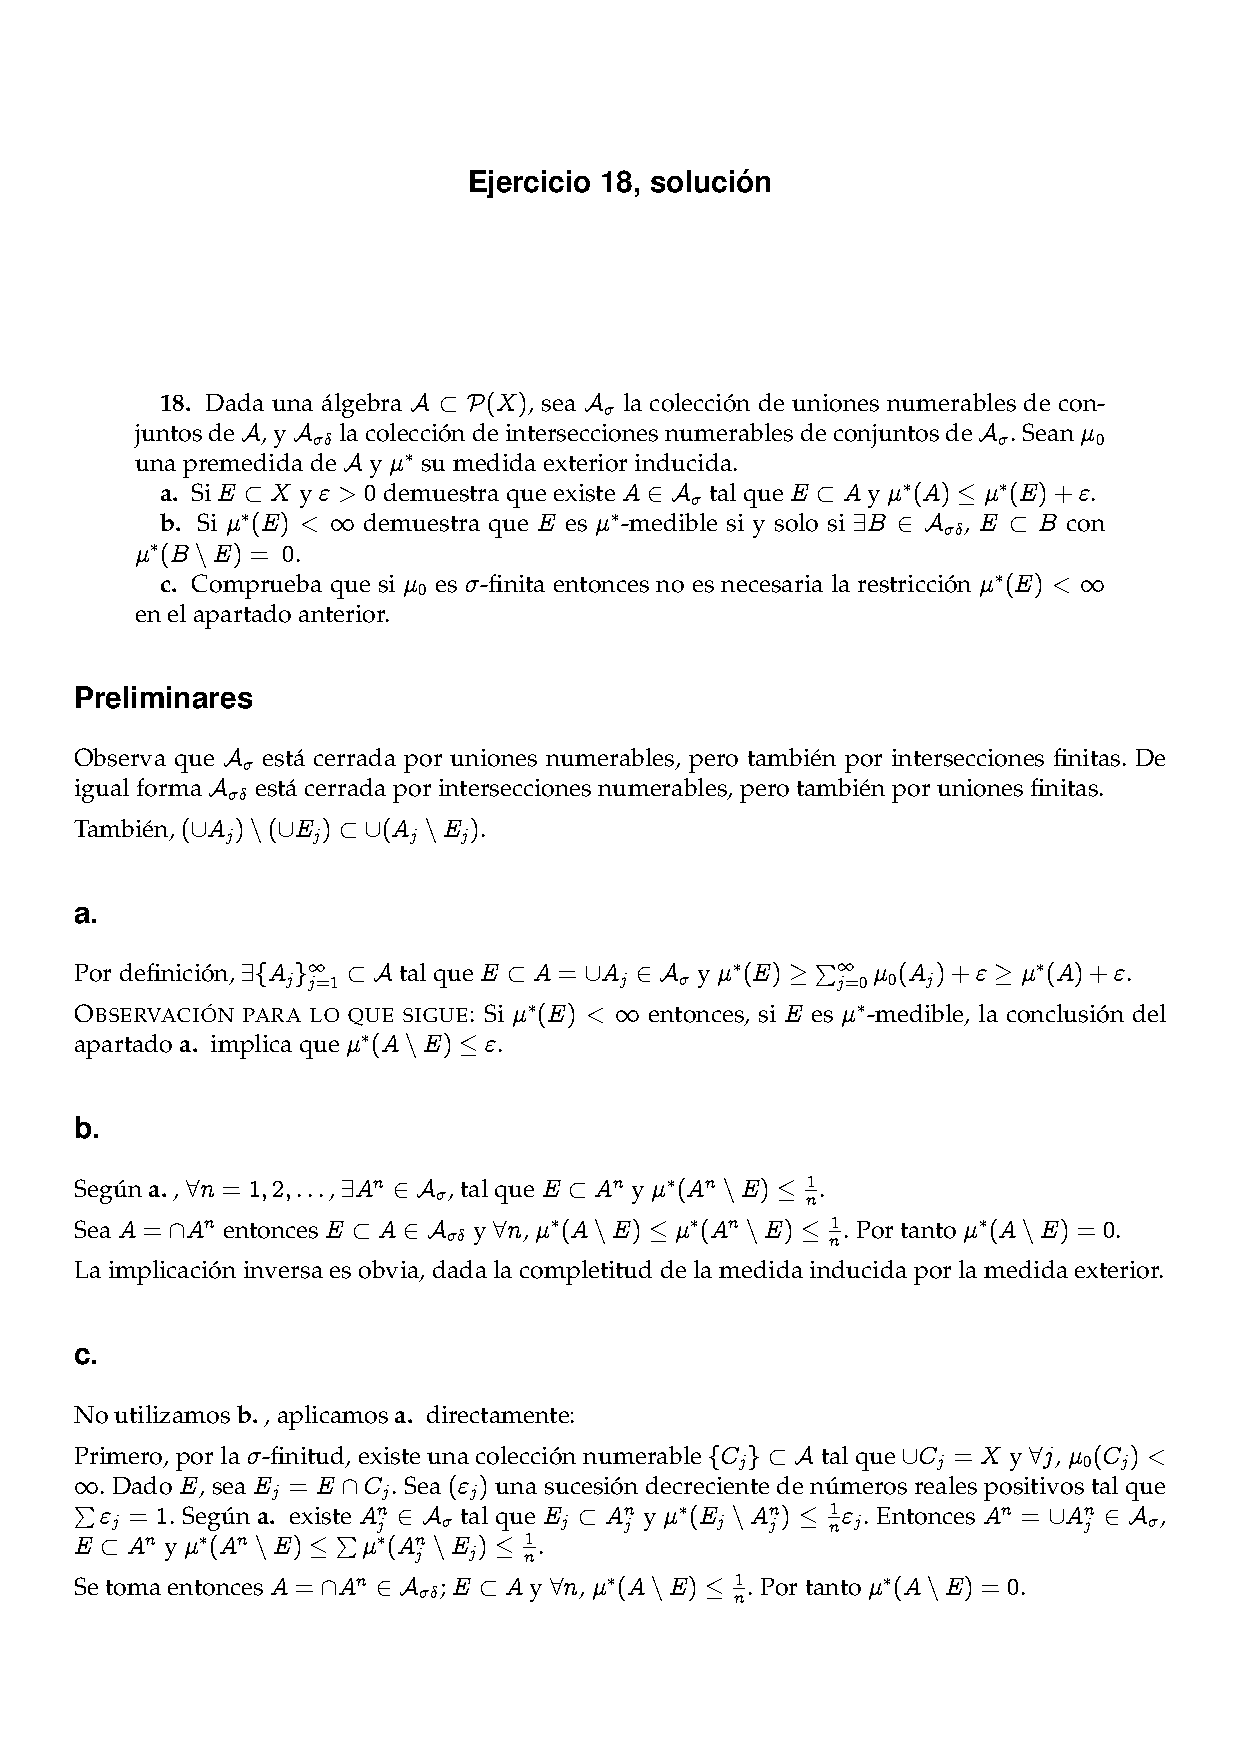
\includepdf[scale=0.9]{pdf/2014-03-18.pdf}
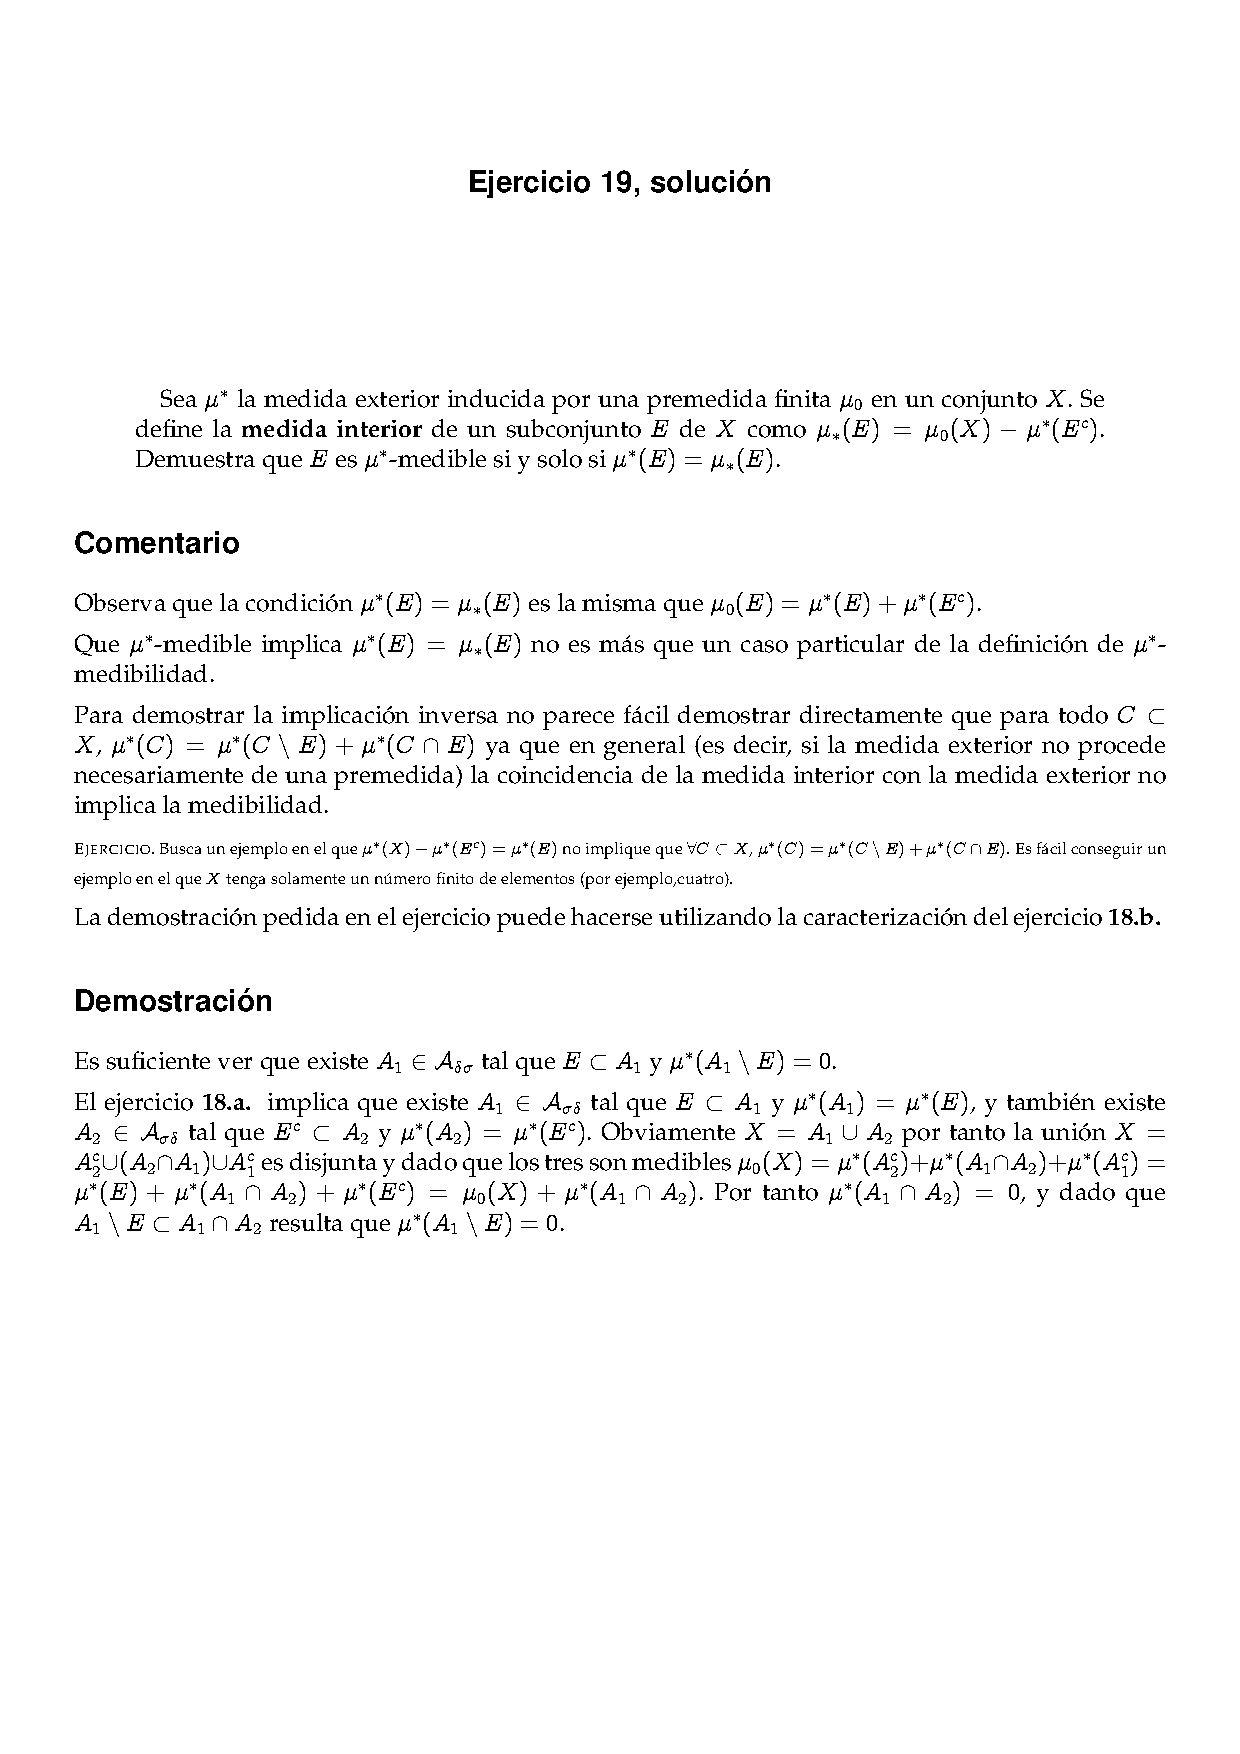
\includepdf[scale=0.9]{pdf/2014-03-19.pdf}
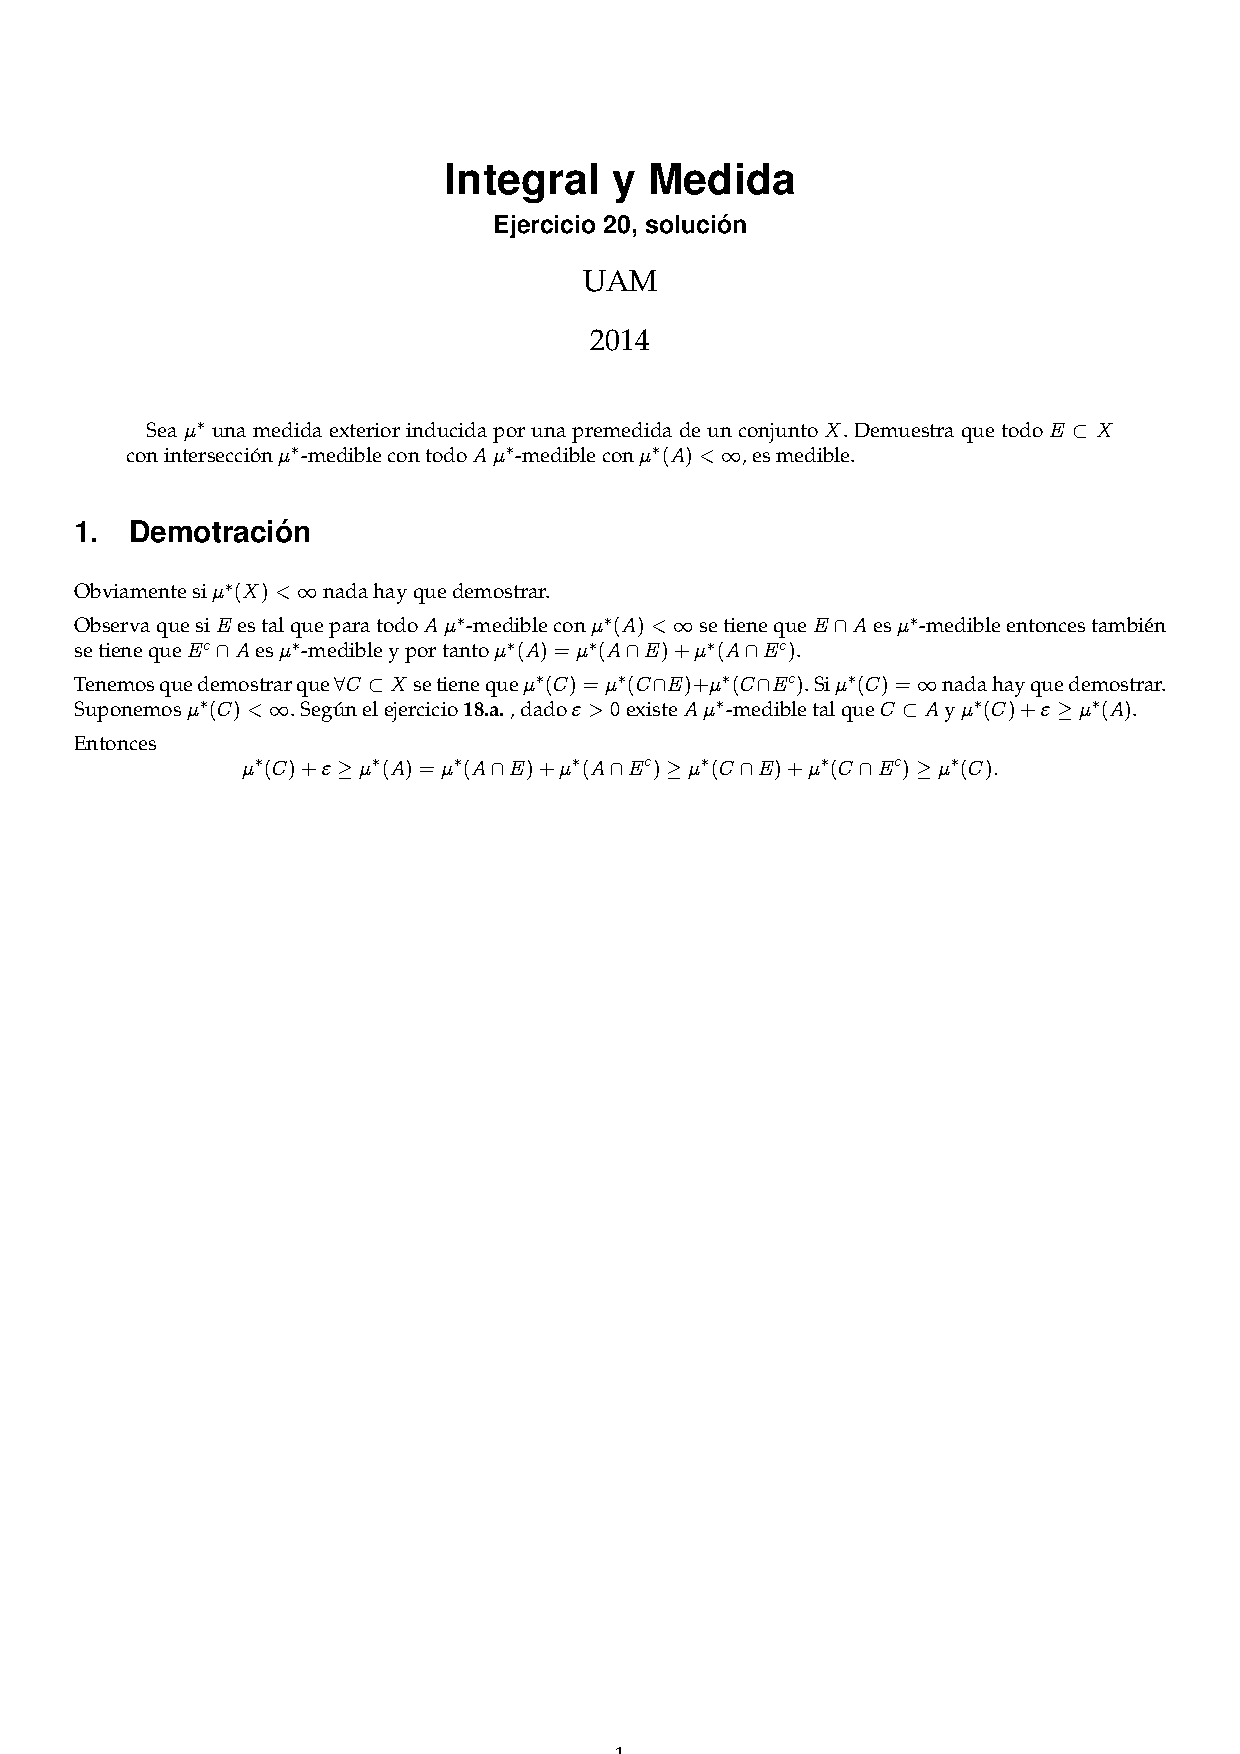
\includepdf[scale=0.9]{pdf/2014-03-20.pdf}

\subsection{Hoja 4}

\begin{problem}
Sea µ la medida de Lebesgue-Stieltjes asociada a la función:
\[F(x)=\left\{ \begin{array}{lcc}
             0 &   \text{si}  & x < 1 \\
             \\ x & \text{si} & 1 \leq x < 3 \\
             \\ 4 &  \text{si}  & 3 \leq x
             \end{array}
   \right.\]

Calcula las siguientes medidas:
\solution
\begin{itemize}
\item $µ(\{1\}) = F(1)-\displaystyle\lim_{x \to 1^-} F(x)$ = 1
\item $µ(\{2\}) = 0$
\item $µ((1, 3]) = F(3)-F(1) = 4 - 1 = 3$
\item $µ((1, 3)) = µ((1, 3]) - µ(\{3\}) = 3 - 1 = 2$
\item $µ([1, 3)) = µ((1, 3)) + µ(\{1\}) = 2 + 1 = 3$
\item $µ([1, 3])) = µ((1, 3]) + µ (\{1\}) = 3 + 1 = 4$
\end{itemize}
\end{problem}

\begin{problem}
Halla funciones de distribución $F$, $F_1$, $F_2$ de forma que, en cada caso, existan $a$ y $b$ tales que:
\begin{enumerate}
\item $µ((a,b)) < F(b)-F(a) < µ([a,b])$, donde $µ=µ_F$
\item $µ_1((a,b)) < µ_1((a,b]) < µ_1([a,b)) < µ_1([a,b])$ y

$µ_2((a,b)) < µ_2([a,b)) < µ_2((a,b]) < µ_2([a,b])$ donde $µ_i = µ_F, \ i=1,2$
\end{enumerate}
\solution
\begin{enumerate}
\item Vale con la función del ejercicio anterior
\item
\textbf{Con i = 1}
\[F_1(x)=\left\{ \begin{array}{lcc}
             0 &   si  & x < 1 \\
             \\ x & si & 1 \leq x < 3 \\
             \\ 3.5 &  si  & 3 \leq x
             \end{array}
   \right.\]

\textbf{Con i = 2}
\[F_2(x)=\left\{ \begin{array}{lcc}
             0 &   si  & x < 1 \\
             \\ x & si & 1 \leq x < 3 \\
             \\ 5 &  si  & 3 \leq x
             \end{array}
   \right.\]
\end{enumerate}

La construcción de estas funciones se ha realizado por la cuenta de la vieja. Si repetimos los cálculos del ejercicio anterior con estas funciones podemos ver que se cumplen las condiciones pedidas (Incluso puede que entendamos de qué va esto)
\end{problem}

\begin{problem}
Sea µ la medida de contar en $(\real, \algbP(\real))$. Para un conjunto finito A $\subset \real$ se define $µ_A(B) = µ(B \cap A)$ para todo $B \subset \real$

\ppart Sea $A=\{1,2,...,n,...\}$ ¿Es $µ_A$ una medida de Lebesgue-Stieltjes?. En caso afirmativo halla $F$ tal que $µ_A=µ_F$
\ppart Sea $A=\{\frac{1}{1},\frac{1}{2},...,\frac{1}{n},...\}$ ¿Es $µ_A$ una medida de Lebesgue-Stieltjes?. En caso afirmativo halla $F$ tal que $µ_A=µ_F$
\solution


\spart Esta medida simplemente cuenta el número de enteros positivos que hay en un conjunto $B$.

Por tanto, simplemente tenemos que buscar una función que realice esa misma función, por ejemplo:
\[F(x)=\left\{ \begin{array}{lcc}
             0 &   si  & 0 \leq x < 1 \\
             \\ n &  si  & n \leq x < n+1
             \end{array}
   \right.\]

Imitando las cuentas realizadas en el ejercicio 1 podemos que ver:
\begin{itemize}
\item $µ((1,3])) = F(3) - F(1) = 2$
\item $µ((1,3)) = µ((1,3])) - µ(\{3\}) = 2 - 1 = 1$
\end{itemize}
observamos que, efectivamente, obtenemos el número de enteros de cada intervalo.

\spart Esta medida cuenta el número de racionales de la forma $\frac{1}{n}$ que hay en un conjunto.

Esta medida no es de Lebesgue-Stieltjes. Una medida de Lebesgue-Stieltjes tiene que tener asociada una función $F$ como en el apartado anterior, es decir, tal que $μ((a,b]) = F(b) - F(a)$, y esta no puede tenerla.

Veamos por qué: tomemos el intervalo $B = (0,ε)$. Su medida según $μ_A$ es infinita, ya que para todo $n$ mayor que $\frac{1}{ε}$, $\frac{1}{n} ∈ A$, y entonces $B∩A$ es infinito. Luego tenemos que encontrar un $F$ tal que $F(ε) - F(0) = ∞$, y la única forma de que eso tenga sentido es que $F(ε) = ∞\; ∀ε$, lo cual es absurdo.

\end{problem}

\begin{problem}
Sea $F$ la función de distribución
\[F(x)=\left\{ \begin{array}{lcc}
             0 &   si  & x \in (-\infty, -1) \\
             \\ 1+x & si & x \in [-1, 0) \\
             \\ 2+x^2 & si & x \in [0, 2) \\
             \\ 9 &  si  & x \in [2, \infty)
             \end{array}
   \right.\]

Siendo $µ=µ_F$, hallar las siguientes medidas.
\solution
\begin{itemize}
\item $µ(\{2\}) = 3 $
\item $µ([-\frac{1}{2}, 3)) = 9 - \frac{1}{2}$
\item $µ((-1,0]\cup (1,2)) = 1 + µ((1,2]) - µ(\{2\}) = 1 + 9 -3 - 3 = 4$
\item $µ([0, \frac{1}{2}) \cup (1, 2]) = \frac{1}{4} + 6$
\item $µ(\{x \in \real \tq |x|+2x^2 > 1\})$=$µ((-\infty, -\frac{1}{2})) + µ((\frac{1}{2}, \infty)) = 0 + 9 - 2 - \frac{1}{4} = 7 - \frac{1}{4}$
\end{itemize}
\end{problem}

\begin{problem}
Sea $\appl{f}{\real}{\real}$ no negativa, integrable Riemann sobre cada intervalo finito y tal que $\int_{-\infty}^{\infty}f(x)=1$.

Prueba que $F(x)=\int_{-\infty}^x f(y) \dif y$ es una función de distribución de probabilidad y que, además, $F$ es continua ($f$ es la función de densidad de $F$).

Si $f(x)=\ind_{[0,1]}$ hallar $F$

\solution
Simplemente tenemos que ver que $F$ es no decreciente, continua por la derecha y que se cumple:
\[\lim_{n \to - \infty}F(x)=0 \ \ \lim_{n \to \infty}F(x)=1\]

Observando que $F$ es una integral y que integrar una función equivale a calcular el área encerrada bajo ella, vemos que a medida que avanzamos la $x$, cada vez estamos calculando un área mayor, luego los dos límites anteriores se cumplen.

Para ver que es continua por la derecha observamos que:
\[ \lim_{h \to 0^+}F(x+h) = \lim_{h \to 0^+} \int_{-\infty}^{x+h}f(y)\dif y = \int_{-\infty}^xf(y)\dif y = F(x)\]

Y es que por ser $F$ una integral, es obvio que es continua.

Suponemos ahora $f(x)=\ind_{[0,1]}$, para responder a la segunda pregunta del enunciado. Entonces
\[F(x)= \int_{-\infty}^{x} \ind_{[0,1]} = \left\{ \begin{array}{lcc}
             0 &   si  & x < 0 \\
             \\ x & si &  0 \leq x \leq 1 \\
             \\ 1 &  si  & 1 \leq x
             \end{array}
   \right.\]
\end{problem}

\begin{problem}
Halla el valor de $k$ para que $f= kx(1-x)\ind_{[0, 1)}$ sea la función de densidad de una medida de probabilidad. Calcula su función de distribución.

\solution
Para que sea función de densidad necesitamos que:
\[\int_{-\infty}^{\infty}f(x) dx = 1\]

Vamos a ver cuánto vale esa integral.
\begin{gather*}
\int_{-\infty}^{\infty}f(x) \dif x = \int_{-\infty}^{\infty}kx(1-x)\ind_{[0, 1)} \dif x  = \\
 = \int_{-\infty}^{0} kx(1-x)\cdot 0 \dif x + \int_{0}^{1}kx(1-x)\dif x + \int_{1}^{\infty}kx(1-x)\cdot 0 \dif x = \\
= k\left(\frac{1}{2}-\frac{1}{3}\right)
\end{gather*}


De donde obtenemos fácilmente que $k = \frac{1}{\frac{1}{2}-\frac{1}{3}} = 6$

La función de distribución sería:
\[\F(x)= \int_{-\infty}^{x} \ind_{[0,1]} = \left\{ \begin{array}{lcc}
             0 &   si  & x < 0 \\
             \\ \int_{0}^{x}kt(1-t)\dif t = (3x^2-2)x^3)& si &  0 \leq x \leq 1 \\
             \\ 1 &  si  & 1 \leq x
             \end{array}
   \right.\]
\end{problem}

\newpage
\begin{problem}
Dado $k$ > 0, sea $f(x)=αe^{-kx}\ind_{[0, \infty)}(x)$
\begin{enumerate}
\item Halla α para que $f$ sea una función de densidad de probabilidad
\item Sea $X$ una variable aleatoria con función de densidad f, si $k=\frac{1}{2}$, calcula la probabilidad de que $X \geq 3$
\item Si $k=\frac{1}{2}$ calcula la probabilidad de que $3 \leq X \leq 6$
\end{enumerate}
\solution
\begin{enumerate}
\item Repitiendo el proceso del ejercicio anterior, debemos hacer que $\int_{0}^{\infty}f(x)dx =1$.

En este caso obtenemos que α=k, es decir, nos encontramos ante una exponencial.

\item
\[\mathbb{P}(X \geq 3) = \int_{³}^{\infty}e^{-kx}dx=e^{\frac{3}{2}}\]

\item Puesto que la función de distribución es continua, la probabilidad de que $X=3$ ó $X=6$ es 0, de modo que podemos calcular la probabilidad pedida como:
\[\mathbb{P}(3 \leq X \leq 6) = \int_{3}^{6}e^{-kx}dx\]
\end{enumerate}
\end{problem}

\begin{problem}
Sea µ la medida de probabilidad definida por la función de distribución:

\[F(x)= \int_{-\infty}^{x} \ind_{[0,1]} = \left\{ \begin{array}{lcc}
             0 &   si  & x \in (- \infty, -1) \\
             \\ \frac{1}{3} & si &  x \in [-1, \sqrt{2}) \\
             \\ \frac{1}{2} + \frac{x-\sqrt{2}}{10} & si &  x \in [\sqrt{2}, 5) \\
             \\ 1 &  si  & x \in [5, \infty)
             \end{array}
   \right.\]

Calcular las siguientes medidas:
\solution

Antes de nada deberíamos comprobar que la función $F(x)$ dada es, efectivamente, una función de distribución. Para ello debemos comprobar que siempre es positiva y que se trata de una función creciente.

En este caso nos fiamos y se deja como ejercicio para el lector desconfiado (Edu) la comprobación de estas propiedades.
\newpage
\begin{enumerate}
\item \[µ((\real \setminus \rac)\cap[\sqrt{2}, 5]) = µ([\sqrt{2}, 5)) = µ((\sqrt{2}, 5]) + µ (\{\sqrt{2}\}) - µ (\{\sqrt{5}\}) =\]
\[ = F(5) - F(\sqrt{2}) +(\frac{1}{2}-\frac{1}{3}) -(1-(1-\frac{\sqrt{2}}{10}))=1-\frac{1}{2}+\frac{1}{6}-\frac{\sqrt{2}}{10}\]

\item \[µ((\real \setminus \rac)\cap [-2, \sqrt{2}]) = µ(\{\sqrt{2}\}) = \frac{1}{2}-\frac{1}{3} = \frac{1}{6}\]

\item \[µ(\rac \cap [1,6]) = µ(\{5\}) = \frac{\sqrt{2}}{10}\]
\end{enumerate}

Vamos ahora a por la parte complicada del ejercicio.

\[A_{3n-2} = \left(\frac{2n}{4n+3}, \frac{4n+5}{3n}\right)\]
\[A_{3n} = \left(\frac{4}{5n+2}, \frac{6n+1}{2n}\right)\]
\[A_{3n-1} = \left(-2, \frac{6n-1}{5n+2}\right)\]

Vemos que:
\begin{enumerate}
	\item $\lim A_{3n-2}= [\frac{1}{2}, \frac{4}{3}]$
	\item $\lim A_n{3n-1} = (-2, \frac{6}{5})$
	\item $\lim A_{3n} = (0^+, 3^+)$
\end{enumerate}

Recordemos que el límite superior de $A_n$ es el conjunto de puntos que están en infinitos conjuntos de la sucesión. Por tanto, todos los puntos contenidos en estos límites se contienen en el límite superior de la sucesión.
\[\limsup A_n = [\frac{1}{2}, \frac{4}{3}] \bigcup  (-2, \frac{6}{5}) \bigcup (0^+, 3^+)\]

Por otro lado, el límite inferior es el conjunto de puntos que se encuentran en todos los elementos de la sucesión a partir de uno dado. Así, el límite inferior será la intersección de los límites calculados anteriormente.
\[\liminf A_n = [\frac{1}{2}, \frac{4}{3}] \bigcap  (-2, \frac{6}{5}) \bigcap (0^+, 3^+)\]

\textcolor{blue}{Completado por mi. No fiarse al 100\%}
\[µ(\limsup A_n) = µ([\frac{1}{2}, \frac{4}{3}]) +  µ((-2, \frac{6}{5})) +µ((0^+, 3^+)) = \frac{1}{3}  + \frac{1}{3} + \frac{1}{3} = 1\]
\[µ(\liminf A_n) = µ([\frac{1}{2}, \frac{6}{5})) = 0\]

\end{problem}

\begin{problem}
Sea $\appl{F}{\real}{\real}$ una función de distribución
\begin{enumerate}
\item Prueba que el conjunto de puntos de discontinuidad de $F$ es numerable
\item Prueba que el conjunto de puntos de continuidad de $F$ es denso en $\real$
\end{enumerate}
\obs $F$ es monótona luego no tiene más discontinuidades que saltos
\solution

\begin{enumerate}
\item Vamos a probar que el número de puntos de discontinuidad en (n, n+1] es numerable.

Para ello tomamos la medida de este intervalo:
\[M = F(n+1)-F(n)\]

La pregunta que nos hacemos ahora es, ¿cuántos puntos $x \in (n, n+1]$ pueden tener $µ_F(\{x\}) \frac{M}{k}$?

La respuesta es sencilla (la supo hasta Elena en clase). $\forall k \in \nat$ No podemos tener más de k puntos con esta condición.

Por tanto no puede haber una cantidad no numerable de puntos de (n, n+1] con $µ_F(\{x\})>0$
%\item Si tuviésemos una cantidad no numerable de discontinuidades tendríamos un intervalo cerrado que contiene una cantidad no numerable de discontinuidades. Puesto que cada una de esas discontinuidades tenemos un salto, resulta que tendríamos un número no numerable de saltos en un intervalo cerrado.

%Así, tendríamos que la medida del intervalo cerrado sería la suma infinita y no numerable de valores positivos, lo que nos daría un resultado finito.

%Leyendo de un artículo de wikipedia:
%\begin{verbatim}
%La suma de los saltos no puede ser mayor que la diferencia de los
%valores de la función en los extremos del intervalo, de modo que
%el conjunto de discontinuidades con salto mayor que 1/n es finito
%y, por tanto, el conjunto de discontinuidades es a lo más numerable
%\end{verbatim}

\item \textcolor{blue}{Hecho por mi. No fiarse al 100\%}

Recordando lo dado en topología, sabemos que un conjunto es denso si la adherencia del conjunto coincide con el total.

Recordamos también que la adeherencia son aquellos puntos tales que todo abierto que lo contenta corta al conjunto dado.

Puesto que las únicas discontinuidades que puede presentar una función de distribución son discontinuidades de salto y es obvio que para cualquier punto en que la función sea continua todo entorno del punto contiene otros puntos de discontinuidad.
\end{enumerate}
\end{problem}

\begin{problem}
Variando si es necesario en cada caso el tamaño de los intervalos, construir un conjunto de tipo Cantor cuya medida de Lebesgue sea mayor que 1-ε
\solution
La construcción del conjunto de Cantor consiste en tomar el intervalo [0,1] y los siguientes conjuntos:
\begin{enumerate}
\item Construimos un intervalo $A_1$ de longitud $\frac{ε}{2}$ centrado en el intervalo [0,1].
\item Construimos $A_2 = \bigcup (a_i, b_i)$ tales que cada elemento de la unión tiene longitud igual a $\frac{1}{2}\frac{ε}{4}$.
\item etc
\end{enumerate}
Así, en el paso n-ésimo tenemos:
\[A_n = (a_1^n,b_1^n) \cup (a_2^n,b_2^n) \cup ... \cup (a_n^n,b_n^n)\]
donde cada intervalo de la unión tiene longitud $\frac{1}{2^{n-1}}\frac{ε}{2}$.

El conjunto de Cantor se obtiene restando del intervalo incial todos los intervalos $A_n$ que hemos ido construyendo. Es decir:
\[C = I -\bigcup A_n\]
\[m(C)=m(I)-\sum m(A_n) = 1 - ε\]
\end{problem}

\begin{problem}
Sea $µ_F$ la medida de Lebesgue-Stieltjes correspondiente a una función creciente y continua $\appl{F}{\real}{\real}$
\begin{enumerate}
\item Prueba que si A es numerable entonces $µ_F(A)$=0
\item Prueba que existen conjuntos A tales que $µ_F(A)> 0$ y A no contiene ningún intervalo abierto.
\item Si $µ(A)\geq 0$ y $µ(\real \setminus A) = 0$, ¿tiene que ser A denso en $\real$
\end{enumerate}
\obs Se recomienda construir una función $F(x)$ que sea constante en un intervalo
\solution

\begin{enumerate}
\item \textcolor{blue}{Hecho por mi. No fiarse al 100\%}

Si $A$ es numerable podemos escribirlo de la forma:
\[A = \bigcup_{i=1}^{\infty}\{a_i\} \tq a_i \neq a_j \forall i, j \ i \neq j\]
por tanto,
\[µ(A) = \sum_{i=1}^{\infty} µ(\{a_i\}) \]
pero, puesto que la función del enunciado es continua, la medida de un único punto siempre es 0 y por lo que
\[µ(A) = \sum_{i=1}^{\infty} µ(\{a_i\}) = \sum_{i=1}^{\infty}  0 = 0\]

\item Podemos tomar el conjunto $(a, b]$ que tendrá
\[µ((a,b]) = F(b)-F(a) \geq 0\]
ya que $F$ es creciente.

Ahora debemos cuida que no contenta abiertos. Para ello basta con tomar la intersección de este intervalo con los racionales.

Con ello eliminamos la posibilidad de que haya abiertos contenidos en el conjunto y mantenemos la medida del conjunto puesto que la medida de los racionales (que son los que estamos extrayendo) es 0.

\item No tiene por qué ser A denso. Pongamos un contraejemplo para probarlo.

Si tomo una función que crece entre el 0 y el 1 y luego se queda constante y tomo $A=(0,1)$ tenemos que se cumplen las condiciones del enunciado pero obviamente el intervalo $(0,1)$ en $\real$ no es denso.
\end{enumerate}
\end{problem}

\begin{problem}
Sea $F(x)=log(1 + |x|)\cdot \ind_{[0, \infty)}(x)$
\begin{enumerate}
\item Comprueba que $\appl{F}{\real}{\real}$ es creciente y continua por la derecha.
\item Calcula $µ_F(\{Cantor\})$
\end{enumerate}
\obs El conjunto de Cantor está contenido en $2^n$ intervalos de longitud $\frac{1}{3^n}$
\solution

\begin{enumerate}
\item \textcolor{blue}{Hecho por mi. No fiarse al 100\%}

Tenemos que ver que $a<b \implies F(a) < F(b)$ lo cual es obvio ya que el logaritmo es creciente y la función indicatriz simplemente vale 0 cuando $x4 < 0$ y 1 en el resto de casos.

Para ver que es contínua por la derecha necesitamos probar que:
\[\lim_{x \to a^+}F(x) = F(a) \ \forall a \in X\]
El único punto donde podemos dudar es en $a=0$ pero en ese caso está claro que:
\[\lim_{x \to 0^+}F(x) = \log(1) = 0 = F(0)\]

\item
\begin{defn}[Conjunto de Cantor]
Es el conjunto de todos los puntos del intervalo real [0,1] que admiten una expresión en base 3 que no utilice el dígito 1
\end{defn}

\[µ_F(\{Cantor\}) = 1 - \frac{1}{3}+2\frac{1}{9}+4\frac{1}{27}+... = \frac{1}{3} \sum_{n=1}^{\infty}\left(\frac{2}{3}\right)^{n-1} = \frac{1}{3} \frac{1}{1-\frac{2}{3}} = 1-1 = 0\]

\end{enumerate}
\end{problem}

\begin{problem}
Sea µ una medida de Borel en $\real$, finita sobre compactos, con $µ((0, 1])=1$
\begin{enumerate}
\item Prueba que si $\forall s \in \real, µ(s + E)=µ(E)$, entonces µ es la medida de Lebesgue.
\item Prueba que si $\forall s \in \real, µ(rE)=|r|µ(E)$, entonces µ es la medida de Lebesgue
\end{enumerate}
\solution
\begin{enumerate}
\item
Para ver que es la medida de Lebesgue necesitamos ver que
\[\forall a,b \ a<b \ µ((a,b]) = b-a\]
Por continuidad podemos restringirnos a trabajar con a,b racionales.

Por la invarianza por traslaciones es suficiente ver:
\[\forall b \in \rac \ µ((0,b])=b\]

Vamos a ello pues
\[µ((0, \frac{p}{q}]) = \sum_{i=1}^{\infty} µ((\frac{1-i}{q}, \frac{i}{q}]) = p\cdot µ((0, \frac{1}{q}])\]

Ahora sólo nos queda ver que $µ((0, \frac{1}{q}]) = \frac{1}{q}$, pero para ello basta con fijarnos en que:
\[µ((0, 1]) = \sum_{i=1}^{\infty} µ((\frac{i-1}{q}, \frac{i}{q}]) = q \cdot µ((0, \frac{1}{q}])\]

\item Se hace prácticamente igual que el apartado anterior. Se deja como ejercicio para casa.


\end{enumerate}
\end{problem}

\begin{problem}
Sea µ la medida de Lebesgue de $\real$ y $E \subset \real$ medible Lebesgue tal que 0 < µ(E) < $\infty$. Demuestra que para todo α, 0<α<1, existe un intervalo abierto I tal que µ($I \cap E$) > α m(I)
\solution
Sabemos que la medida de Lebesgue se puede aproximar bien por abiertos que contengan al conjunto $E$, es decir:
\[\forall ε > 0 \ \exists A \text{ abierto con } E \subset A \tq µ(E) > µ(A)-ε \]

Tomamos $A= \bigcup_{k=1}^{\infty} I_k$ con los $I_k$ disjuntos.

Suponemos ahora que $\exists α \in (0,1) \tq \forall I \text{ intervalo abierto } µ(E \cap I)\leq αµ(I)$
Entonces
\[µ(E) = \sum_{k=1}^{\infty}µ(E \cap I_k) \leq \sum_{k=1}^{\infty} α µ(I_k) = α µ(A)\]

Si la suposición fuese cierta tendríamos ahora
\[µ(A)-µ(E) \geq µ(A) - α µ(A) (1-α)µ(A) \geq (1-α)µ(E) > ε\]
y llegamos a contradicción.
\end{problem}



%% Apéndices (ejercicios, exámenes)
\appendix



% Bibliografia
\newpage
\begin{thebibliography}{}
	D. R. Stinson, "Cryptography: Theory and Practice" (Básica)

	
\end{thebibliography}

\printindex
\end{document}
